\documentclass{ximera}

\begin{document}
	\author{Stitz-Zeager}
	\xmtitle{TITLE}


\mfpicnumber{1}

\opengraphsfile{IntroLimits}

\setcounter{footnote}{0}

\label{IntroLimits}

In this chapter, we take some more steps towards\footnote{into?} Calculus.  We first revisit the  concept of \index{limit}\textbf{limit} .  We've primarily used limits as a way to analyze and codify function behavior in places where we simplify could not evaluate the function.\footnote{Whether it be describing end behavior as $x \rightarrow  - \infty$  or $x \rightarrow  \infty$ or places where we'd be dividing by `$0$.'}  We first focus on how the concept is expressed graphically.

\subsection{Limits from Graphs}
\label{limitsfromgraphs}

Even though we didn't introduce the limit concept or notation until Chapter \ref{PolynomialFunctions}, we first encounter the underlying concept much earlier.  Recall in  Example \ref{functiongraphex01} we were given the graph of a function $w = F(v)$:

\begin{center}

\begin{tikzpicture}[scale=0.8]
  % Axes
  \draw[->] (-5,0) -- (5.2,0) node[below right] {\scriptsize $v$};
  \draw[->] (0,-5) -- (0,5.2) node[above right] {\scriptsize $w$};

  % Axis ticks
  \foreach \x in {-4,-3,-2,-1,1,2,3,4}
    \draw (\x,0.1) -- (\x,-0.1);
  \foreach \y in {-4,-3,-2,-1,1,2,3,4}
    \draw (0.1,\y) -- (-0.1,\y);

  % Custom x-axis labels
  \node[below] at (-1,0) {\scriptsize $-1$};
  \node[below] at (1,0)  {\scriptsize $1$};
  \node[below] at (4,0)  {\scriptsize $4$};

  % Custom y-axis labels
  \node[left] at (0,-3) {\scriptsize $-3$};
  \node[left] at (0,-2) {\scriptsize $-2$};
  \node[left] at (0,-1) {\scriptsize $-1$};
  \node[left] at (0,1)  {\scriptsize $1$};
  \node[left] at (0,2)  {\scriptsize $2$};
  \node[left] at (0,3)  {\scriptsize $3$};
  \node[left] at (0,4)  {\scriptsize $4$};

  % Labels for specific points
  \node[below] at (2,0) {\scriptsize $(2,0)$};
  \node[below] at (-2,0) {\scriptsize $(-2,0)$};
  \node[below] at (0,-4) {\scriptsize $(0,-4)$};
  \node[below right] at (1,-3) {\scriptsize $(1,-3)$};

  % Function plot: w = v^2 - 4
  \draw[thick,domain=-2:3,samples=100] plot (\x,{\x*\x-4});

  % Points
  \filldraw ( -2, 0) circle (2pt);
  \filldraw (  0,-4) circle (2pt);
  \filldraw (  2, 0) circle (2pt);

  \draw (1,-3) circle (2pt); % unfilled point
\end{tikzpicture}

% \begin{mfpic}[15]{-5}{5}{-5}{5}
% \axes
% \tlabel[cc](5,-0.5){\scriptsize $v$}
% \tlabel[cc](0.5,5){\scriptsize $w$}
% \tlabel[cc](2.5,-0.5){\scriptsize $(2,0)$}
% \tlabel[cc](-3,-0.5){\scriptsize $(-2,0)$}
% \tlabel[cc](1,-4.25){\scriptsize $(0,-4)$}
% \tlabel[cc](2,-3.25){\scriptsize $(1,-3)$}
% \xmarks{-4 step 1 until 4 }
% \ymarks{-4 step 1 until 4}
% \tlpointsep{5pt}
% \scriptsize
% \axislabels {x}{{$-1 \hspace{7pt}$} -1, {$1$} 1, {$4$} 4}
% \axislabels {y}{{$-3$} -3,{$-2$} -2,  {$-1$} -1, {$1$} 1, {$2$} 2, {$3$} 3, {$4$} 4}
% \normalsize
% \penwd{1.25pt}
% \arrow \function{-2,3,0.1}{x**2-4}
% \point[4pt]{(-2,0), (0,-4), (2,0)}
% \pointfillfalse
% \point[4pt]{(1,-3)}
% \end{mfpic} 

\end{center}


The hole in the graph tells us that even though $F(1)$ is undefined, we'd \textbf{expect} $F(1)$ to be $-3$ based on what's happening with the graph \textbf{near} the point $(1,-3)$.  Using limit notation, we'd write  $\ds{\lim_{v \rightarrow 1} F(v) = -3}$.  We take a moment below to better define what we mean when use the limit notation.

\medskip

\colorbox{ResultColor}{\bbm

\begin{defn} \label{informallimitdefn} \textbf{Informal Definition of Limit:}  Given a function $f$ defined on an open interval containing $x=a$, except possibly at $x=a$, the notation $\ds{\lim_{x \rightarrow a} f(x) = L}$,\index{limit ! informal definition} means as input values, $x$, approach\footnote{ignoring what is happening at $x=a$} the number $a$, the output values, $f(x)$, approach the number $L$.  The notation ` $\ds{\lim_{x \rightarrow a} f(x) = L}$'  is read read `the \textbf{limit} as $x$ approaches $a$ of $f(x)$ equals $L$.' 
\end{defn}

\ebm}


\medskip


Some remarks about Definition \ref{informallimitdefn} are in order.  Note that the business about $f$ being defined on `an open interval containing $x=a$'  is there to guarantee that we have the appropriate `room' for inputs $x$ to approach $a$ from either direction.\footnote{We'll get to `one-sided' limits here shortly.}  (For now, we'll just assume we all understand what the word `approach' means in this context and let a Calculus class explain how this is more precisely codified mathematically.)

\medskip 

The phrase  `except possibly at $x=a$' which immediately follows means the limit doesn't concern itself with what is actually happening at $x=a$.  The function  $f$ may or may not be defined at $x = a$.  Indeed,  if  $\ds{\lim_{x \rightarrow a} f(x) = L}$, $f(a)$ could be $L$, $f(a)$  could be a number different than $L$ or $f(a)$ could not be defined. 

\medskip

 This drives home the principle difference between the precalculus notion of `$f(a)$' and the Calculus notion of  `$\ds{\lim_{x \rightarrow a} f(x)}$':  `$\ds{\lim_{x \rightarrow a} f(x)}$' is what we \textbf{expect} $f(a)$ to be - which may or may not agree with what $f(a)$, if $f(a)$ is even defined. 

\medskip

For example, using the graph from Example \ref{functiongraphex01}, we write $\ds{\lim_{v \rightarrow 0} F(v) = -4}$ since as $v \rightarrow 0$, we see $w = F(v) \rightarrow -4$.  In this particular case, $F(0) = -4$ so we get from $F$ at $v=0$ what we expect to get.\footnote{This is another way to describe the notion of \index{continuity}\textbf{continuity}.  (See Definition \ref{continuousdefn}.)}

\medskip

For another example, consider the graphs of the functions $f$, $g$, and $h$ below near $x = 2$. Through a precalculus lens, each of these functions is different at $x = 2$:   $f(2) = 3$, $g(2) = 1$, and $h(2)$ is undefined.  Through a Calculus lens, however, all three of these functions are behaving identically as  $x$ approaches $2$:   $\ds{\lim_{x \rightarrow 2} f(x) = 3}$, $\ds{ \lim_{x \rightarrow 2} g(x)= 3}$, and $\ds{\lim_{x \rightarrow 2} h(x) = 3}$.


\begin{center}

\begin{tabular}{ccc}

 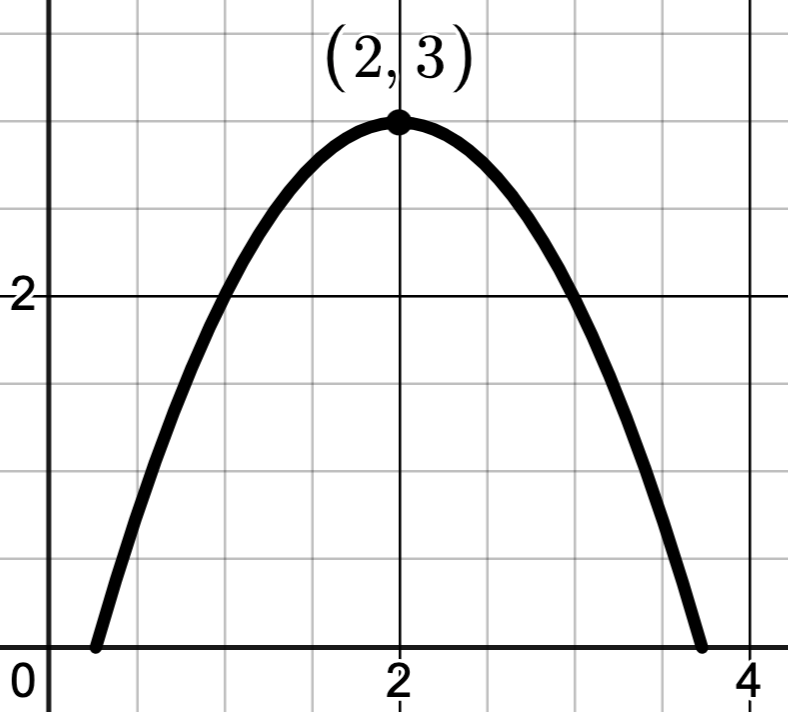
\includegraphics[width=2in]{./IntroLimitsGraphics/limitgrapha.png} &  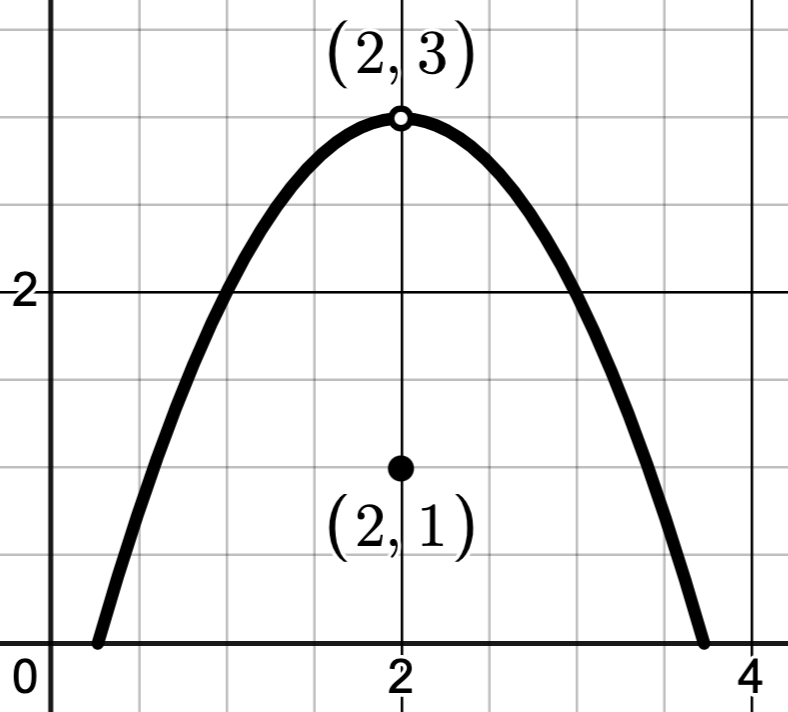
\includegraphics[width=2in]{./IntroLimitsGraphics/limitgraphc.png} &  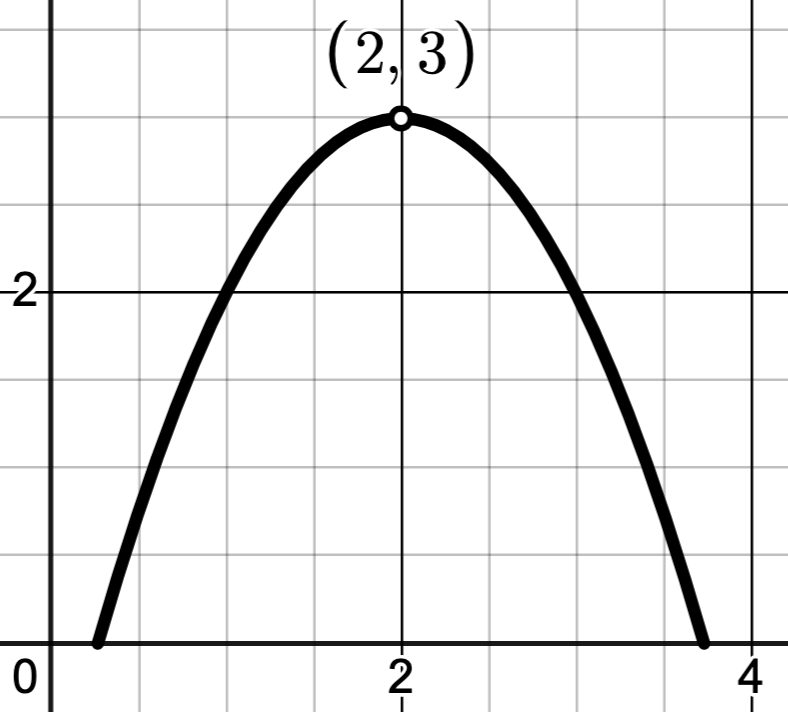
\includegraphics[width=2in]{./IntroLimitsGraphics/limitgraphb.png} \\
 
 $y = f(x)$ & $y = g(x)$ & $y = h(x)$ \\
 
 \end{tabular}
 
 \end{center}
 

 Next let's head to Section \ref{ConstantandLinearFunctions} and revisit Example \ref{piecewiseconstantex} in a piecewise-defined function is used to model matinee admission prices at a local theater:
    
   \begin{center}

\begin{mfpic}[25]{-1}{6}{-1}{5}
\axes
\tlabel[cc](6,-0.5){\scriptsize $A$}
\tlabel[cc](0.5,5){\scriptsize $y$}
\xmarks{1,2,3,4,5}
\ymarks{1,2,3,4}
\scriptsize
\tlabel[cc](-1, 2.875){$(0, 5.75)$}
\tlabel[cc](0.8, 4){$(6, 7.25)$}
\tlabel[cc](5, 2.5){$(50, 5.75)$}
\tlpointsep{4pt}
\axislabels {x}{ {$10$} 1, {$20$} 2, {$30$} 3, {$40$} 4, {$50$} 5}
\axislabels {y}{{$2$} 1, {$4$} 2,   {$8$} 4}
\penwd{1.25pt}
\polyline{( 0,2.875), (0.6,2.875)}
\polyline{( 0.6,3.625), (5,3.625)}
\arrow \polyline{(5,2.875), (6, 2.875)}
\point[3pt]{(0,2.875), (5, 2.875),( 0.6,3.625) }
\pointfillfalse
\point[3pt]{(0.6,2.875), (5,3.625)}
\tcaption{ $y = p(A) = \begin{mycases} 
      5.75 &  \text{if $0 \leq A < 6$ or $A \geq 50$} \\
      7.25  & \text{if $6 \leq A < 50$} \\
   \end{mycases}$}
\normalsize
\end{mfpic} 

\end{center}

What can be said about $\ds{ \lim_{A \rightarrow 6} p(A)}$?   Remember, $\ds{ \lim_{A \rightarrow 6} p(A)}$ is what we would \textbf{expect} $p(6)$ to be by analyzing $p$ as $A \rightarrow  6$, ignoring what is happening at $A=6$.  If $A<6$,  $p(A)$ is always $5.75$, so, based on this information, we'd \textbf{expect} $p(6)$ to be $5.75$.   If $A>6$, then  $p(A)$ is always $7.25$, so we'd \text{expect} $p(6)$ to be $7.25$.  Since Definition  \ref{informallimitdefn} requires the $p(A)$ values to approach a \textbf{single} value $L$ as $A \rightarrow 6$, we'd say in this case that   $\ds{ \lim_{A \rightarrow 6} p(A)}$ does not exist.  

\medskip

Even though $\ds{ \lim_{A \rightarrow 6} p(A)}$ does not exist, we've used so-called `one-sided' limit notation in Chapters \ref{RationalFunctions} and \ref{RootRadicalPowerFunctions} which we can apply here.  Specifically, we write  $\ds{\lim_{A \rightarrow 6^{-}} p(A) = 5.75}$ and  $\ds{\lim_{A \rightarrow 6^{+}} p(A) = 7.25}$ to more precisely record the behavior of $p$ as we approach $ A = 6$ from either direction.\footnote{Note that $\ds{\lim_{A \rightarrow 6^{+}} p(A) = 7.25 = p(6)}$ in this case.  So at least we `get' what we `expect to get' when approaching $6$ from the right.}

\medskip

\colorbox{ResultColor}{\bbm

\begin{defn} \label{onesidedimitdefn} \textbf{One-sided Limits:}  

\begin{itemize}

\item If $f$ is defined on an open interval for $x<a$ except possibly at $x=a$, the notation  $\ds{\lim_{x \rightarrow a^{-}} f(x) = L}$,\index{limit ! informal definition ! from the left} read `the \textbf{limit} as $x$ approaches $a$ \textbf{from the left} of $f(x)$ equals $L$' means as input values, $x$, $x < a$, approach the number $a$ (ignoring what is happening at $x=a$), the output values, $f(x)$, approach the number $L$. 

\item If $f$ is defined on an open interval for $x>a$ except possibly at $x=a$, the notation  $\ds{\lim_{x \rightarrow a^{+}} f(x) = L}$,\index{limit ! informal definition ! from the right} read `the \textbf{limit} as $x$ approaches $a$ \textbf{from the right} of $f(x)$ equals $L$' means as input values, $x$, $x > a$, approach the number $a$ (ignoring what is happening at $x=a$), the output values, $f(x)$, approach the number $L$. 


\end{itemize}

\end{defn}

\ebm}


\medskip

In order for the (two-sided) limit to exist, both one-sided limits need to exist, be equal, and vice-versa.  This is recorded in the following theorem.

\medskip

\colorbox{ResultColor}{\bbm

\begin{thm}  \label{onesidedlimit}  Given a function $f$ defined on an open interval containing $x=a$, except possibly at $x=a$,  $\ds{\lim_{x \rightarrow a} f(x) = L}$ if and only if $\ds{\lim_{x \rightarrow a^{-}} f(x) = L}$ and $\ds{\lim_{x \rightarrow a^{+}} f(x) = L}$.


\end{thm}
\ebm}

\medskip

It's time for an example.

\begin{ex} \label{limitfromgraphex} Use the \textbf{complete} graph\footnote{Recall this means this is the entire graph of $f$.  There's nothing hidden offscreen.} of $y = f(x)$ below to answer the following questions.





\begin{center}

 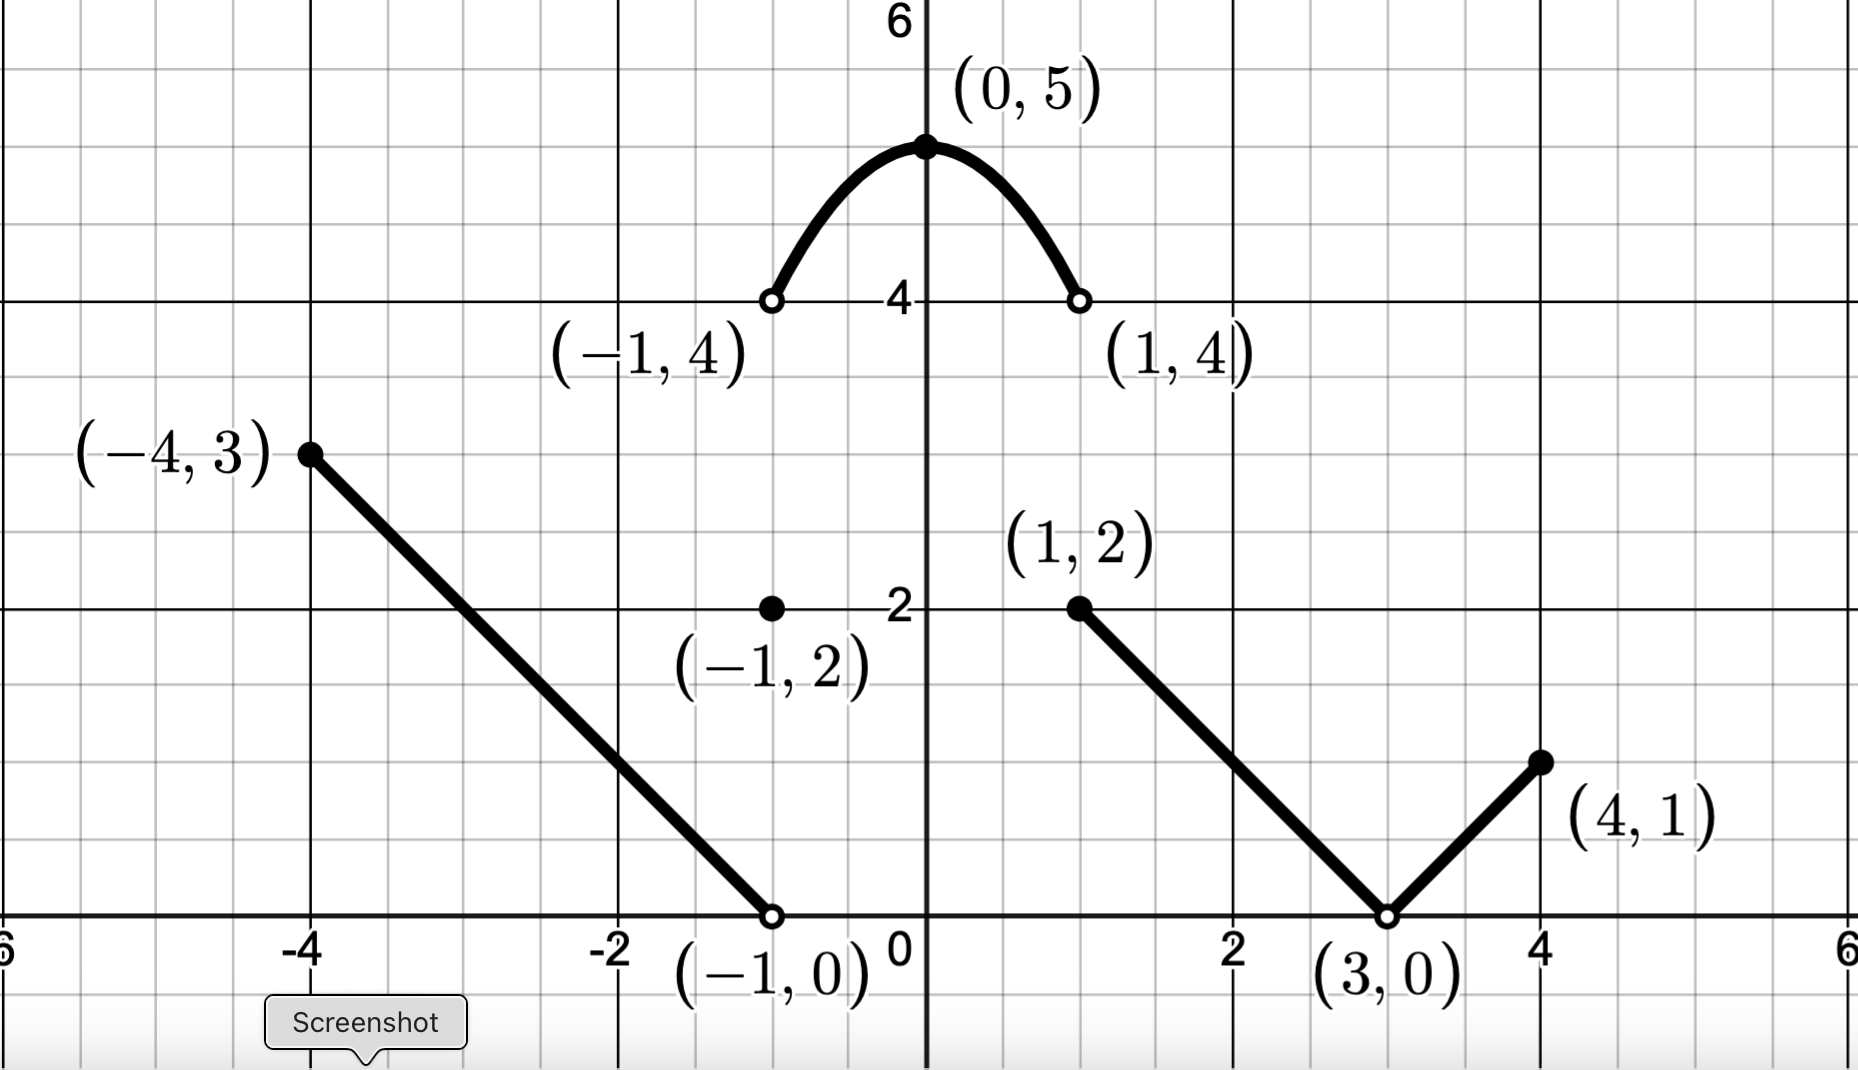
\includegraphics[width=5.5in]{./IntroLimitsGraphics/LimitfromGraphEx.png}
 
  \end{center}
  
  

  
  
\begin{enumerate}

\item  State the domain and range of $f$ using interval notation.


\item  Find the following values. Explain your reasoning.

 \begin{multicols}{4}
 
 \begin{itemize}
 
 \item $f(-1)$
 
 \item  $\ds{ \lim_{x \rightarrow -1^{-}} f(x)}$
 
  \item  $\ds{ \lim_{x \rightarrow -1^{+}} f(x)}$
 
  \item  $\ds{ \lim_{x \rightarrow -1} f(x)}$
 
 \end{itemize}
 
  \end{multicols}
 
\smallskip
 
  \begin{multicols}{4}
 
 \begin{itemize}
 
 \item $f(1)$
 
 \item  $\ds{ \lim_{x \rightarrow 1^{-}} f(x)}$
 
  \item  $\ds{ \lim_{x \rightarrow 1^{+}} f(x)}$
 
   \item  $\ds{ \lim_{x \rightarrow 1} f(x)}$
 
 \end{itemize}
 
  \end{multicols}
 
\smallskip
 
 \begin{multicols}{4}
 
 \begin{itemize}
 
 \item $f(0)$
 
 \item  $\ds{ \lim_{x \rightarrow 0^{-}} f(x)}$
 
  \item  $\ds{ \lim_{x \rightarrow 0^{+}} f(x)}$
 
  \item  $\ds{ \lim_{x \rightarrow 0} f(x)}$
 
 \end{itemize}
 
  \end{multicols}
 
\smallskip
 
  \begin{multicols}{4}
 
 \begin{itemize}
 
 \item $f(3)$
 
 \item  $\ds{ \lim_{x \rightarrow 3^{-}} f(x)}$
 
  \item  $\ds{ \lim_{x \rightarrow 3^{+}} f(x)}$
 
   \item  $\ds{ \lim_{x \rightarrow 3} f(x)}$
 
 \end{itemize}
 
  \end{multicols}
 
\smallskip

\item  Explain why  $\ds{ \lim_{x \rightarrow -4} f(x)}$ does not exist and find  $\ds{ \lim_{x \rightarrow -4^{+}} f(x)}$
\smallskip

\item  Explain why  $\ds{ \lim_{x \rightarrow 4} f(x)}$ does not exist and find  $\ds{ \lim_{x \rightarrow 4^{-}} f(x)}$

\end{enumerate}


{\bf Solution.}

\begin{enumerate}

\item  Projecting the graph of $f$ to the $x-$axis, we find that everything from $-4$ to $4$, inclusive, is covered except for $x = 3$.  Hence the domain is $[-4,3) \cup (3,4]$.  When projecting the graph of $f$ to the $y$-axis, we see everything between $0$ and $3$ is covered (excluding $0$ and including $3$) then everything between $4$  and $5$ is covered (excluding $4$ and including $5$).  Hence the range is $(0,3] \cup (4,5]$.


\item  \begin{itemize}  \item  Regarding $x = -1$:  since the point $(-1,2)$ is on the graph of $f$, we know $f(-1) =2$.  To determine  $\ds{ \lim_{x \rightarrow -1^{-}} f(x)}$, we see that the graph to the left of $x = -1$ is headed towards the point $(-1,0)$ as $x$ approaches $-1$.  Hence,  $\ds{ \lim_{x \rightarrow -1^{-}} f(x)= 0}$.  To determine  $\ds{ \lim_{x \rightarrow -1^{+}} f(x)}$, we see that the graph to the right of $x = -1$  is headed towards the point $(-1,4)$ as $x$ approaches $-1$.  Hence,  $\ds{ \lim_{x \rightarrow -1^{+}} f(x)= 4}$.    Since $\ds{ \lim_{x \rightarrow -1^{-}} f(x)}$ and $\ds{ \lim_{x \rightarrow -1^{+}} f(x)}$ are different,  $\ds{ \lim_{x \rightarrow -1} f(x)}$ does not exist.

\item  Regarding $x = 1$:  since the point $(1,2)$ is on the graph of $f$, we know $f(1) =2$.  To determine  $\ds{ \lim_{x \rightarrow 1^{-}} f(x)}$, we see that the graph to the left of $x = 1$ is headed towards the point $(1,4)$ as $x$ approaches $1$.  Hence,  $\ds{ \lim_{x \rightarrow 1^{-}} f(x)= 4}$.  To determine  $\ds{ \lim_{x \rightarrow 1^{+}} f(x)}$, we see that the graph to the right of $x = 1$  is headed towards the point $(1,2)$ as $x$ approaches $1$.  Hence,  $\ds{ \lim_{x \rightarrow 1^{+}} f(x)= 2}$.    Since $\ds{ \lim_{x \rightarrow 1^{-}} f(x)}$ and $\ds{ \lim_{x \rightarrow 1^{+}} f(x)}$ are different,  $\ds{ \lim_{x \rightarrow 1} f(x)}$ does not exist.

\item  Regarding $x = 0$:  since the point $(0,5)$ is on the graph of $f$, we know $f(0) =5$.  To determine  $\ds{ \lim_{x \rightarrow 0^{-}} f(x)}$, we see that the graph to the left of $x = 0$ is headed towards the point $(0,5)$ as $x$ approaches $0$.  Hence,  $\ds{ \lim_{x \rightarrow 0^{-}} f(x)= 5}$.  To determine  $\ds{ \lim_{x \rightarrow 0^{+}} f(x)}$, we see that the graph to the right of $x = 0$  is headed towards the point $(0,5)$ as $x$ approaches $0$.  Hence,  $\ds{ \lim_{x \rightarrow 0^{+}} f(x)= 5}$.    Since $\ds{ \lim_{x \rightarrow 0^{-}} f(x)}$ and $\ds{ \lim_{x \rightarrow 0^{+}} f(x)}$ are both $5$,  $\ds{ \lim_{x \rightarrow 0} f(x) = 5}$.


\item  Regarding $x = 3$:  since there is no point on the graph of $f$ with an $x$-coordinate of $3$, $f(3)$ is undefined.  To determine  $\ds{ \lim_{x \rightarrow 3^{-}} f(x)}$, we see that the graph to the left of $x = 3$ is headed towards the point $(3,0)$ as $x$ approaches $3$.  Hence,  $\ds{ \lim_{x \rightarrow 3^{-}} f(x)= 0}$.  To determine  $\ds{ \lim_{x \rightarrow 3^{+}} f(x)}$, we see that the graph to the right of $x = 3$  is headed towards the point $(3,0)$ as $x$ approaches $3$.  Hence,  $\ds{ \lim_{x \rightarrow 3^{+}} f(x)= 0}$.    Since $\ds{ \lim_{x \rightarrow 3^{-}} f(x)}$ and $\ds{ \lim_{x \rightarrow 3^{+}} f(x)}$ are both $0$,  $\ds{ \lim_{x \rightarrow 3} f(x) = 0}$.

\end{itemize}

\item In order to find   $\ds{ \lim_{x \rightarrow -4} f(x)}$, we need to analyze the graph of $f$ from both the left an right of $x=-4$.  Since there is no graph to the left of $x = -4$,  $\ds{ \lim_{x \rightarrow -4^{-}} f(x)}$, and hence $\ds{ \lim_{x \rightarrow -4} f(x)}$ does not exist.  However, $\ds{ \lim_{x \rightarrow -4^{+}} f(x) = 3}$, since, when coming from the right, the graph approaches the point $(-4,3)$ as $x$ approaches $-4$.


\item In order to find  $\ds{ \lim_{x \rightarrow 4} f(x)}$, we need to analyze the graph of $f$ from both the left an right of $x=4$.  Since there is no graph to the right of $x = 4$,  $\ds{ \lim_{x \rightarrow 4^{+}} f(x)}$, and hence $\ds{ \lim_{x \rightarrow 4} f(x)}$ does not exist.  However, $\ds{ \lim_{x \rightarrow 4^{-}} f(x) = 1}$, since, when coming from the left, the graph approaches the point $(4,1)$ as $x$ approaches $4$.  \qed


\end{enumerate}

\end{ex}


Another use of limits we've seen is to codify unbounded behavior.  Since $\infty$ and $-\infty$ aren't real numbers,  we used limit notation to help us describe end behavior  (as $x \rightarrow - \infty$ or $x \rightarrow \infty$) and unbounded function behavior ($f(x)\rightarrow -\infty$ or $f(x) \rightarrow \infty$.)  Let's take a moment to think about what it means to write $\ds{\lim_{x \rightarrow \infty} f(x) = \infty}$.  How does one `approach' infinity anyhow?  

\medskip

Let's consider  $\ds{\lim_{x \rightarrow \infty} x^2 = \infty}$.  What me mean here is that as $x$ grows larger and larger (without bound), $f(x) = x^2$ follows suit.  To prove something like this, we'd need to show that for any `arbitrarily large' real number, $N$, we can find some threshold $M$ so that if the inputs, $x>M$, the outputs, $f(x) > N$.  For example, if we set $N = 10000$, then to guarantee $f(x) = x^2 > 10000$, we can solve and get $x > \sqrt{10000} = 100$.  So provided $x > 100$, $f(x) > 10000$.  In this case, $N = 10000$ and $M = \sqrt{10000} = 100$.  In general, if $x > \sqrt{N}$, $x^2 > N$, which justifies us writing $\ds{\lim_{x \rightarrow \infty} x^2 = \infty}$.

\medskip

We can adjust the inequality signs in the sort of argument\footnote{If this sort of argument seems familiar, it should!  Replacing `$>$' with `$=$' is how we proved the ranges  of the monomial functions and Laurent monomials  in Sections \ref{GraphsofPolynomials} and \ref{IntroRational}, respectively.}   above to direct $x$ or $f(x)$ to either $\infty$ or $-\infty$.  Doing so gives us the (formal) definitions of below.

\medskip


\colorbox{ResultColor}{\bbm

\begin{defn}  \label{infinitelimitsatinfinity}  $~$

\begin{enumerate}

\item  Given a function $f$ defined on an open interval  $(a, \infty)$:

\begin{itemize}

\item   the notation `$\ds{\lim_{x \rightarrow \infty} f(x) = \infty}$' means that for any real number $N$ there is a real number $M$ so that if $x > M$, $f(x) > N$.

\item   the notation `$\ds{\lim_{x \rightarrow \infty} f(x) = -\infty}$' means that for any real number $N$ there is a real number $M$ so that if $x > M$, $f(x) < N$.

\end{itemize}

\item  Given a function $f$ defined on an open interval  $(-\infty, a)$:

\begin{itemize}

\item   the notation `$\ds{\lim_{x \rightarrow -\infty} f(x) = \infty}$' means that for any real number $N$ there is a real number $M$ so that if $x < M$, $f(x) > N$.

\item   the notation `$\ds{\lim_{x \rightarrow -\infty} f(x) = -\infty}$' means that for any real number $N$ there is a real number $M$ so that if $x < M$, $f(x) < N$.

\end{itemize}

\end{enumerate}

\end{defn}
\ebm}

\medskip

We'll explore Definition \ref{infinitelimitsatinfinity} more in the Exercises. In the meantime, the reader is encouraged to take some time and think about the inequalities in Definition \ref{infinitelimitsatinfinity} and how they force the corresponding graphical behavior showcased below:

\begin{center}

\begin{tabular}{cccc}

\begin{mfpic}[25][15]{-1}{3}{-1}{5.5}

\axes
\tlabel[cc](3,-0.5){\scriptsize $x$}
\tlabel[cc](0.5,5.5){\scriptsize $y$}
\penwd{1.25pt}
\arrow \function{1,2.2,0.1}{2*x}
\end{mfpic} 

& 

\begin{mfpic}[25][15]{-1}{3}{-5.5}{1}

\axes
\tlabel[cc](3,-0.5){\scriptsize $x$}
\tlabel[cc](0.5,1){\scriptsize $y$}
\penwd{1.25pt}
\arrow \function{1,2.2,0.1}{0-2*x}
\end{mfpic} 

& 


\begin{mfpic}[25][15]{-3}{1}{-1}{5.5}

\axes
\tlabel[cc](1,-0.5){\scriptsize $x$}
\tlabel[cc](0.5,5.5){\scriptsize $y$}
\penwd{1.25pt}
\arrow \reverse \function{-2.2,-1,0.1}{0-2*x}
\end{mfpic}  

&


\begin{mfpic}[25][15]{-3}{1}{-5.5}{1}

\axes
\tlabel[cc](1,-0.5){\scriptsize $x$}
\tlabel[cc](0.5,1){\scriptsize $y$}
\penwd{1.25pt}
\arrow \reverse \function{-2.2,-1,0.1}{2*x}
\end{mfpic}  \\


$\ds{\lim_{x \rightarrow \infty} f(x)  = \infty}$

&

$\ds{\lim_{x \rightarrow \infty} f(x)  = -\infty}$

&

$\ds{\lim_{x \rightarrow -\infty} f(x)  = \infty}$

&

$\ds{\lim_{x \rightarrow -\infty} f(x)  = -\infty}$ \\



\end{tabular}

\end{center}


Combining the ideas of what it means for $x$ or $f(x)$ to approach (finite) real numbers along with our (more precise notion) of what it means for $x$ or $f(x)$ to approach $-\infty$ or $\infty$, we can mix and match to produce expressions and graphs containing vertical and horizontal asymptotes such as the ones depicted below:


\begin{center}

\begin{tabular}{ccc}


\begin{mfpic}[15][8]{-1}{6}{-1}{9}
\axes
\dashed \polyline{(5, 2), (5,9)}
\scriptsize
\tlabel[cc](6, -0.5){$x$}
\tlabel[cc](0.5, 9){$y$}
%\tlabel[cc](-0.75, 0.5){$(0,4)$}
%\tlabel[cc](3, 1.25){$\left(4 ,100 \right)$}
\tlabel[cc](5, 1){$x = 5$}
\normalsize
\penwd{1.25pt}
\arrow \function{0, 4.666,0.1}{1/((x-5)**2)}
%\point[4pt]{(0,0.01), (4,1)}
%\tcaption{\scriptsize $y =P(t)$}
\end{mfpic}

&

\begin{mfpic}[15][8]{-5}{5}{-9}{1}
\axes
\scriptsize
\tlabel[cc](5, -0.5){$x$}
\tlabel[cc](0.5, 1){$y$}
%\tlabel[cc](-2, 1){$(-1,1)$}
%\tlabel[cc](2, 1){$(1,1)$}
\normalsize
\penwd{1.25pt}
\arrow \reverse \arrow \function{-5,-0.3333,0.1}{0-1/(x**2)}
\arrow \reverse \arrow \function{0.3333,5,0.1}{0-1/(x**2)}
%\point[4pt]{(-1,1), (1,1)}
%\tcaption{\scriptsize $y = \frac{1}{t^2}$}
\end{mfpic}
 &
 
 \begin{mfpic}[15][8]{-1}{9}{-1}{9}
\axes
\dashed \polyline{(-1,5), (9,5)}
\scriptsize
\tlabel[cc](9, -0.5){$x$}
\tlabel[cc](0.5, 9){$y$}
\tlabel[cc](7, 5.5){$y = 3$}
%\tlabel[cc](-1, 0.5){$(0,50)$}
%\tlabel[cc](1.75, 3.25){$\left(\frac{2}{3},350 \right)$}
\normalsize
\penwd{1.25pt}
\arrow \function{0,9,0.1}{5 - (1.5/(x+1/3))}
%\point[4pt]{(0,0.5), (0.6666,3.5)}
%\tcaption{\scriptsize $y=N(t)$}
\end{mfpic}
 
  \\


 $\ds{\lim_{x \rightarrow 5^{-} }f(x) = \infty}$ &  $\ds{\lim_{x \rightarrow 0} f(x) = - \infty}$ &  $\ds{\lim_{x \rightarrow \infty} f(x) = 3}$ \\
 
 \end{tabular}
 
 \end{center}


We would be remiss in our duties as (pre)Calculus instructors if we failed to point out that even though we've  used notation `$= \infty$'  in expressions like $\ds{\lim_{x \rightarrow 5^{-} }f(x) = \infty}$ above, since $\infty$ is not a real number, technically, $\ds{\lim_{x \rightarrow 5^{-} }f(x)}$ does not exist.  The  `$= \infty$' here just codifies better \textbf{the manner in which} the limit fails to exist.

\medskip

Our last example of this section turns the tables and has you construct the graph of function given information provided by limits.


\begin{ex} \label{graphfromlimits} Sketch the graph of a function $f$ which satisfies all of the following criteria:

\begin{center}


\begin{multicols}{3}

\begin{itemize}

\item $\ds{\lim_{x \rightarrow -\infty} f(x) = 0}$

\item $\ds{\lim_{x \rightarrow -1^{-}} f(x) = \infty}$

\item $\ds{\lim_{x \rightarrow -1^{+}} f(x) = - \infty}$


\end{itemize}

\end{multicols}

\begin{multicols}{3}

\begin{itemize}


\item $\ds{\lim_{x \rightarrow 1^{-}} f(x) = -\frac{1}{2}}$ 

\item $\ds{\lim_{x \rightarrow 1^{+}} f(x) = 0}$ 


\item  $\ds{\lim_{x \rightarrow \infty } f(x) = \infty}$  \\

\end{itemize}

\end{multicols}




\end{center}

The sign diagram for $f$ is:

\begin{center}

\begin{mfpic}[15]{-5}{5}{-5}{6}
\arrow \reverse \arrow \polyline{(-5,0),(5,0)}
\xmarks{-2,2}
\tcaption{A sign diagram for $f(x)$}
\tlpointsep{4pt}
\axislabels {x}{{$-1 \hspace{7pt}$} -2, {$1$} 2}
\tlabel[cc](-3.5,1){$(+)$}
\tlabel[cc](-2,1){\textinterrobang}
\tlabel[cc](0,1){$(-)$}
\tlabel[cc](2,1){$0$}
\tlabel[cc](3.5,1){$(+)$}
\end{mfpic}


\end{center}



{\bf Solution.} Each piece of information given describes a portion of the graph of $y = f(x)$.  The strategy is to sketch each individual portion and connect them together.

\medskip

First off, $\ds{\lim_{x \rightarrow -\infty} f(x) = 0}$ tells us that $y = 0$ is a horizontal asymptote to the graph.  This means as we head off to the left, the graph approaches the $x$-axis.  Since the sign diagram tells is $f(x) > 0$ for $x<-1$, we know the graph must approach the $x$-axis from above.

\medskip

Next, we have $\ds{\lim_{x \rightarrow -1^{-}} f(x) = \infty}$ and  $\ds{\lim_{x \rightarrow -1^{+}} f(x) = - \infty}$ which tells us $x=-1$ is a vertical asymptote to the graph.  These behaviors agree with the sign diagram both in sign (`$+$' $\infty$ for $x<-1$ and `$-$' $\infty$ for $x>-1$) and the fact that $f$ is undefined at $x = -1$.

\medskip

Moving on we are given information about $f$ near $x = 1$.    The limit $\ds{\lim_{x \rightarrow 1^{-}} f(x)}$ $= -\frac{1}{2}$  means as we approach $x=1$ from the left, the $y$-values approach $-\frac{1}{2}$.  Likewise, $\ds{\lim_{x \rightarrow 1^{+}} f(x) = 0}$ means as we approach $x=1$ from the right, the $y$-values approach $0$ (the $x$-axis).  

\medskip

The sign diagram tells us that, indeed, $f(1) = 0$.  Hence, as $x \rightarrow 1^{-}$,  the graph of $f$ approaches a hole at $\left(0, -\frac{1}{2}\right)$.  As $x \rightarrow 0^{+}$, the graph of $f$ approaches an $x$-intercept, $(1,0)$, which is included in the graph. 

\medskip

Finally,   $\ds{\lim_{x \rightarrow \infty } f(x) = \infty}$  means that as we move farther to the right, the graph moves farther up which we indicate, as usual, with an arrow up to the right.

\medskip

Connecting these pieces together (careful to not violate the Vertical Line Test, Theorem \ref{VLT}) we get:

\begin{center}


\begin{mfpic}[20][60]{-6}{5}{-2}{2}
\dashed \polyline{(-1,-2), (-1,2)}
%\point[4pt]{(0,-0.333)}
\tlabel[cc](5,0.1){\scriptsize $x$}
\tlabel[cc](0.5,2){\scriptsize $y$}
\tlabel[cc](2.25,-0.5){\scriptsize $\left(1, -\frac{1}{2} \right)$}
\axes
\xmarks{-5 step 1 until 4}
\ymarks{-1.5 step 0.5 until 1.5}
\tiny
\tlpointsep{4pt}
\axislabels {x}{{$-5 \hspace{7pt}$} -5, {$-4 \hspace{7pt}$} -4, {$-3 \hspace{7pt}$} -3, {$-2 \hspace{7pt}$} -2, {$-1\hspace{7pt}$} -1, {$1$} 1, {$2$} 2, {$3$} 3, {$4$} 4}
\axislabels {y}{{$-1$} -1, {$1$} 1}
\normalsize
\penwd{1.25pt}
\arrow \reverse \arrow \function{-6,-1.5,0.1}{-1/(x+1)}
\arrow \reverse \function{-0.5,1,0.1}{-1/(x+1)}
\arrow \function{1,4,0.1}{(x**2)/8 - 1/8}
\point[4pt]{(1, 0)}
\pointfillfalse
\point[4pt]{(1, -0.5)}
\end{mfpic}


\end{center}

\hfill \qed

\end{ex}





\subsection{Limit Properties and an Introduction to Continuity}
\label{LimitPropertiesandContinuity}

Let  $f(x) = 6$.  Consider $\ds{\lim_{x \rightarrow 5} f(x)  =  \lim_{x \rightarrow 5} 6}$.   Since the function values are unchanging, there is no other value other than `$6$' to expect from $f$ so it stands to reason that $\ds{\lim_{x \rightarrow 5} f(x)  =  \lim_{x \rightarrow 5} 6 = 6}$. Indeed, for any real number $a$,  $\ds{\lim_{x \rightarrow a} 6  = 6}$.   In general, if $f(x) = c$ is a constant function, $\ds{\lim_{x \rightarrow a} f(x) =   \lim_{x \rightarrow a} c = c}$.  The formal proof of this fact requires a formal definition of limit,but for now, we'll just take it as true.

\medskip

Next, let's consider $f(x) = x$.  Consider $\ds{\lim_{x \rightarrow 5} f(x) = \lim_{x \rightarrow 5} x }$. What do we expect the value of `$x$' to be as $x \rightarrow 5$?  Well, `$5$'.  Indeed, it can be proved that $\ds{\lim_{x \rightarrow a} x = a}$ for all real numbers, $a$.


\medskip

What about $\ds{\lim_{x \rightarrow 5}  (x+6)}$?  Since $\ds{\lim_{x \rightarrow 5} x = 5}$ and $\ds{ \lim_{x \rightarrow 5} 6 = 6}$, it stands to reason that \[\ds{\lim_{x \rightarrow 5}  (x+6) = \lim_{x \rightarrow 5} x  + \lim_{x \rightarrow 5} 6 = 5 + 6 = 11,}\] which is indeed the case.  It turns out that in most cases, limits do respect arithmetic:
\medskip

\colorbox{ResultColor}{\bbm

\begin{thm}  \label{LimitProp01}  \textbf{(Some of the) Properties of Limits:}

\begin{enumerate}

\item  \textbf{Constant Rule:} If $c$ is a constant, then $\ds{ \lim_{x \rightarrow a} c = c}$ for every real number $a$.

\item \textbf{Identity Rule:} $\ds{ \lim_{x \rightarrow a} x = a}$ for every real number $a$.

\item  \textbf{Limits Respect Function Arithmetic:}  If $\ds{ \lim_{x \rightarrow a} f(x) = L}$ and $\ds{ \lim_{x \rightarrow a} g(x) = K}$, then:

\begin{enumerate}

\item \textbf{Sum and Difference Rule:}  $\ds{\lim_{x \rightarrow a} \left[f(x)\pm g(x)\right] =
\lim_{x \rightarrow a} f(x) \pm \lim_{x \rightarrow a} g(x) = L
\pm K}$

\item \textbf{Product Rule:}  $\ds{\lim_{x \rightarrow a} \left[f(x) \, g(x)\right] =
\left[\lim_{x \rightarrow a} f(x)\right] \, \left[ \lim_{x
\rightarrow a} g(x)\right] = L \, K}$

\begin{enumerate}

\item \textbf{Scalar Multiple Rule:}  If $c$ is a real number, $\ds{\lim_{x \rightarrow a} \left[c \, f(x)\right] =
c \, \left[\lim_{x \rightarrow a} f(x)\right] =c \, L}$


\item \textbf{Power Rule:}  If   $n$ is any
natural number,\footnote{Recall this means  $n = 1,2,3,\ldots$}
$\ds{\lim_{x \rightarrow a} \left[f(x)\right]^{n} = \left[
\lim_{x \rightarrow a} f(x) \right]^{n}= L^{n}}$.
\end{enumerate}

\item \textbf{Quotient Rule:}  $\ds{\lim_{x \rightarrow a} \left[ \frac{f(x)}{g(x)}\right]
= \frac{\ds{\lim_{x \rightarrow a} f(x)}} { \ds{\lim_{x
\rightarrow a} g(x)}} = \frac{L}{K}}$, provided $K \neq 0$.

\item \textbf{Rules for Radicals:}  

\begin{itemize}

\item If $n$ is \textbf{odd}, $\ds{\lim_{x \rightarrow a} \sqrt[n]{f(x)} = \sqrt[n]{\lim_{x \rightarrow a} f(x)} = \sqrt[n]{L}} $. 

\item  If $n$ is \textbf{even} and $L>0$, $\ds{\lim_{x \rightarrow a} \sqrt[n]{f(x)} = \sqrt[n]{\lim_{x \rightarrow a} f(x)} = \sqrt[n]{L}} $. 

\item  If $n$ is \textbf{even} and $L=0$, $\ds{\lim_{x \rightarrow a} \sqrt[n]{f(x)} = 0}$ provided $f(x) \geq 0$ for all $x$ near $a$.
 
 \end{itemize}
 
 \item \textbf{Real Number Powers:}  If $L>0$ and $p$ is a real number, $\ds{\lim_{x \rightarrow a} [f(x)]^{p} = \left[\lim_{x \rightarrow a} f(x)\right]^{p} = L^{p}} $.
 

\end{enumerate}


\end{enumerate}

\end{thm}
\ebm}

\medskip

For those interested, the Scalar Multiple Rule and Power Rule are grouped with the Product Rule since they both follow directly from the Product Rule.  For instance, using the Product Rule,  \[ \lim_{x \rightarrow a} \left[c \, f(x)\right] = \lim_{x \rightarrow a} c \, \lim_{x \rightarrow a}  f(x) = c \, \lim_{x \rightarrow a}  f(x).\]  For powers, note that $\left[f(x)\right]^2 = f(x)  \, f(x) $ so that \[ \lim_{x \rightarrow a} \left[ f(x)\right]^2 = \lim_{x \rightarrow a} \left[ f(x) \, f(x) \right] =  \lim_{x \rightarrow a} f(x)  \, \lim_{x \rightarrow a}  f(x) = L \, L = L^2.\]  Once this is established, we can use the fact that $\left[f(x)\right]^3 = f(x)  \, \left[f(x)\right]^2 $ and the product rule again to get \[ \lim_{x \rightarrow a} \left[ f(x)\right]^3 = \lim_{x \rightarrow a} \left[ f(x) \, \left[f(x)\right]^2 \right] =  \lim_{x \rightarrow a} f(x)  \, \lim_{x \rightarrow a}  \left[f(x)\right]^2= L \, L^2 = L^3.\] Continuing in this manner gives us the Power Rule.\footnote{See Exercise \ref{limitpowerruleproof} in Section \ref{Induction} for more details.}

\medskip

A note regarding the Rules for Radicals:  since $\sqrt{N}$ is not real  if $N<0$, we have to be careful about limits involving even-indexed radicals (or exponents which indicate even-indexed radicals.)   For example, consider $\ds{\lim_{x \rightarrow 5} \sqrt{5-x}}$.  Since this is a `two-sided' limit, we must consider both $x \rightarrow 5^{-}$ and $x \rightarrow 5^{+}$.

\medskip

As $x \rightarrow 5^{-}$, the radicand, $(5-x) >0$ so $\sqrt{5-x}$ is defined as a real number.  More specifically, as $x \rightarrow 5^{-}$, the quantity $(5-x) \rightarrow 0^{+}$ so $\ds{\lim_{x \rightarrow 5^{-}} \sqrt{5-x} = 0}$.  On the other hand, if $x \rightarrow 5^{+}$, the quantity $(5-x) < 0$, and $\sqrt{5-x}$ is no longer a real number.  Therefore, $\ds{\lim_{x \rightarrow 5^{+}} \sqrt{5-x}}$, and, hence, $\ds{\lim_{x \rightarrow 5} \sqrt{5-x}}$ does not exist.

\medskip

Note the Real Number Powers rule can be thought as a generalization of the Power Rule, Quotient Rule, and  Rules for Radicals for the case $L>0$. Recall that positive rational number exponents can be defined in terms of natural number powers and radicals as:  $x^{\frac{m}{n}} = \left( \sqrt[n]{x}\right)^{m}$.  Negative exponents can be defined in terms of quotients:  $x^{-\frac{m}{n}} = \frac{1}{x^{\frac{m}{n}}}$.  For the Real Number Exponents rule, we are generalizing the exponents to any real number but keeping the stipulation that $L>0$ to make sure the resulting answer is defined.\footnote{See the discussion of real number exponents in  Section \ref{PowerFunctions}.}

\medskip

We put the limit properties to good use in the following example.

\pagebreak

\begin{ex} \label{limitpropex} Let $f(x)=  \dfrac{ x \sqrt{x+1}}{x^2+2x-4}$.  Use Theorem \ref{LimitProp01} to find $\ds{\lim_{x \rightarrow 3} f(x) }$.

\medskip


{\bf Solution.}

\[ \begin{array}{rclr}

\ds{\lim_{x \rightarrow 3} \dfrac{ x \sqrt{x+1}}{x^2+2x-4}} & = &  \ds{\dfrac{\lim_{x \rightarrow 3} x \sqrt{x+1} }{\lim_{x \rightarrow 3} \left(x^2+2x-4\right)}}  & \text{Quotient Rule }  \\ 

&&&\\
                                                                                           & = &  \ds{  \dfrac{ \left( \lim_{x \rightarrow 3} x \right) \left(  \lim_{x \rightarrow 3} \sqrt{x+1} \right) }{\lim_{x \rightarrow 3} \left( x^2 \right) +\lim_{x \rightarrow 3} ( 2x ) - \lim_{x \rightarrow 3} 4 }}  & \dfrac{\text{Product Rule}}{\text{Sum and Difference Rule}}  \\ 

&&& \\

 & = &  \ds{  \dfrac{ 3   \, \sqrt{ \lim_{x \rightarrow 3} (x+1) } }{ \left( \lim_{x \rightarrow 3}  x \right)^2  +2 \, \lim_{x \rightarrow 3} x  -4 }}  & \dfrac{\text{Identity and Radical Rules}}{\text{Power, Constant Multiple, and Constant Rules}}  \\ 
 
 &&& \\

 & = &  \ds{  \dfrac{ 3   \, \sqrt{ \lim_{x \rightarrow 3} x+\lim_{x \rightarrow 3} 1  } }{ (3)^2  +2 (3)   -4 }}  & \dfrac{\text{Sum Rule }}{\text{Identity Rule }}  \\ 
 
 
 &&& \\

 & = &  \ds{  \dfrac{ 3   \, \sqrt{ 3+ 1  } }{ 9+6   -4 } = \dfrac{6}{11} }  & \text{Identity and Constant Rules, Simplify \hfill $\qed$}  \\ 

\end{array} \] 

\end{ex}

\medskip

It is worth noting that we could have arrived at the same (correct) answer to Example \ref{limitpropex} by evaluating $f(3)$:  $f(3) = \frac{ 3   \, \sqrt{ 3+ 1  } }{ (3)^2+6   -4 } = \frac{6}{11}$.  That's really the power of Theorem \ref{LimitProp01}.  Under `nice' circumstances,\footnote{primarily those in which we're not dealing with piecewise-defined functions or dividing by $0$ \ldots}  Theorem \ref{LimitProp01} allows us to compute limits using direct substitution.  Functions with this property have a  familiar name.

\medskip



\colorbox{ResultColor}{\bbm

\begin{defn}\index{continuous ! limit definition}  \label{continuousdefn}  A function $f$ is said to be \textbf{continuous} at an input $x  = a$ if $\ds{\lim_{x \rightarrow a} f(x) = f(a)}$.  

\medskip

Said differently, a function $f$ is said to be continuous at a real number $a$ if what we \textbf{get}, $f(a)$, exactly what we \textbf{expect to get}, $\ds{\lim_{x \rightarrow a} f(x)}$. 


\end{defn}

\ebm}

\medskip

 This is not the first time we've mentioned this property of functions.  Indeed, we've discussed continuity albeit in graphical terms throughout Chapters \ref{IntroductiontoFunctions} through \ref{RootRadicalPowerFunctions}.  In those chapters, we described continuous functions as those whose graphs are connected meaning they have  `no holes or breaks' in them.  It is a great exercise to compare the description given in Definition \ref{continuousdefn} to the graphical description to see how those two ideas mesh.
 
 \medskip
 
 In a standard Calculus course, you'll explore properties of continuous functions more extensively.  For our purposes here, polynomial, and, more generally, rational functions are continuous \textbf{on their domains}, as well as the functions we encountered in Chapter \ref{RootRadicalPowerFunctions}.  Indeed, so long as we avoid the usual domain pitfalls, combining continuous functions via the standard four operation function arithmetic or using function composition results in a continuous function.  This means in order to \textbf{evaluate limits} of these functions, we may use Definition \ref{continuousdefn} and simply \textbf{evaluate the function} at the corresponding value.

\pagebreak

\begin{ex} \label{piecewisecontex}    Let $f(x) = \begin{mycases}  2x-1 &  \text{if $x  < 2$}  \\  x^2   & \text{if $x \geq 2$} \\  \end{mycases}$.

\begin{enumerate}

\item Is $f$ is continuous at $x = 2$?    Explain.

\item  Find a constant `$m$' so that $g(x) = \begin{mycases}  m \, x-1 &  \text{if $x  < 2$}  \\  x^2   & \text{if $x \geq 2$} \\  \end{mycases}$ is continuous at $x = 2$.

\end{enumerate}

{\bf Solution.}

\begin{enumerate}

\item To determine if $f$ is continuous at $x=2$, we need to check to see if $\ds{\lim_{x \rightarrow 2} f(x) = f(2)}$.   We note that $f$ is defined at $x=2$ and that  $f(2) = (2)^2 = 4$ so we set about determining  $\ds{\lim_{x \rightarrow 2} f(x)}$.  

\medskip

Since $f$ is a piecewise-defined function which has different formulas on either side of $2$, we need to check $\ds{\lim_{x \rightarrow 2} f(x)}$ from both directions.  To find $\ds{\lim_{x \rightarrow 2^{-}} f(x)}$, we note that as $x\rightarrow 2^{-}$, $x < 2$ so $f(x) = 2x-1$.  Hence, $\ds{\lim_{x \rightarrow 2^{-}} f(x) = \lim_{x \rightarrow 2^{-}} (2x-1) = 2(2)-1 = 3}$, the last step coming from the fact that for $x<2$, $f(x) = 2x-1$ is a linear function (a polynomial)  and is continuous.  

\medskip

Now on to  $\ds{\lim_{x \rightarrow 2^{+}} f(x)}$.  Here, $x\rightarrow 2^{+}$, so $x > 2$ and  $f(x) = x^2$.  Hence, $\ds{\lim_{x \rightarrow 2^{+}} f(x) = \lim_{x \rightarrow 2^{+}} x^2 = (2)^2 = 4}$,  the last step courtesy of the fact that for $x>2$,  $f(x) = x^2$ is a quadratic function (a polynomial) and is continuous.  

\medskip

Since $\ds{\lim_{x \rightarrow 2^{-}} f(x) = 3}$ and $\ds{\lim_{x \rightarrow 2^{+}} f(x) = 4}$, we have that $\ds{\lim_{x \rightarrow 2} f(x)}$ does not exist per Theorem \ref{onesidedlimit}.  Hence, $f$ is not continuous.  If we graph $f$ near $x=2$ using desmos, we can see the vertical gap or `jump' occurring at $x = 2$.  

\medskip

\item In this problem,\footnote{For a graphically interactive take on this problem, check out this \href{https://www.desmos.com/calculator/ibtrzesg4i}{\underline{desmos worksheet}}.}  we're given a parameter `$m$' to help us adjust the left hand side of the graph to meet the right hand side at $x = 2$.  If $x<2$, $g(x) = mx-1$ so $\ds{\lim_{x \rightarrow 2^{-}} g(x) = \lim_{x \rightarrow 2^{-}} (mx-1) = 2m-1}$. 

\medskip

To ensure the limit exists, we need  $\ds{\lim_{x \rightarrow 2^{-}} g(x) = \lim_{x \rightarrow 2^{+}} g(x)}$.  Since $g(x) = f(x) = x^2$ for $x \geq 2$, we know $\ds{ \lim_{x \rightarrow 2^{+}} g(x) = 4}$.  Solving  $2m-1 = 4$, we get $m = \frac{5}{2} = 2.5$.  Sure enough, $\ds{\lim_{x \rightarrow 2^{-}} (2.5x-1) = 5 - 1 = 4}$.  Since $g(2) = 4$, we have $\ds{\lim_{x \rightarrow 2} g(x) = g(2)}$, so $g$ is continuous at $x = 2$. 

\begin{center}

\begin{tabular}{cc}

 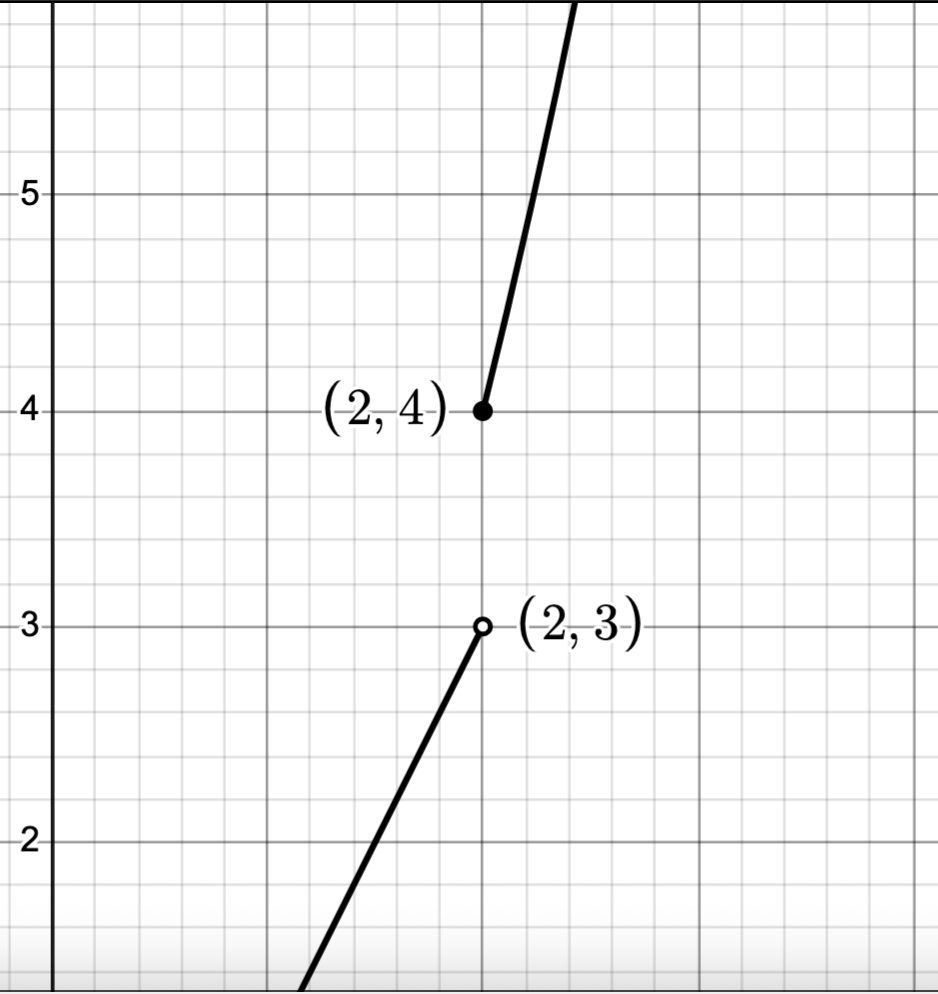
\includegraphics[width=3in]{./IntroLimitsGraphics/jumpdisc.png} &  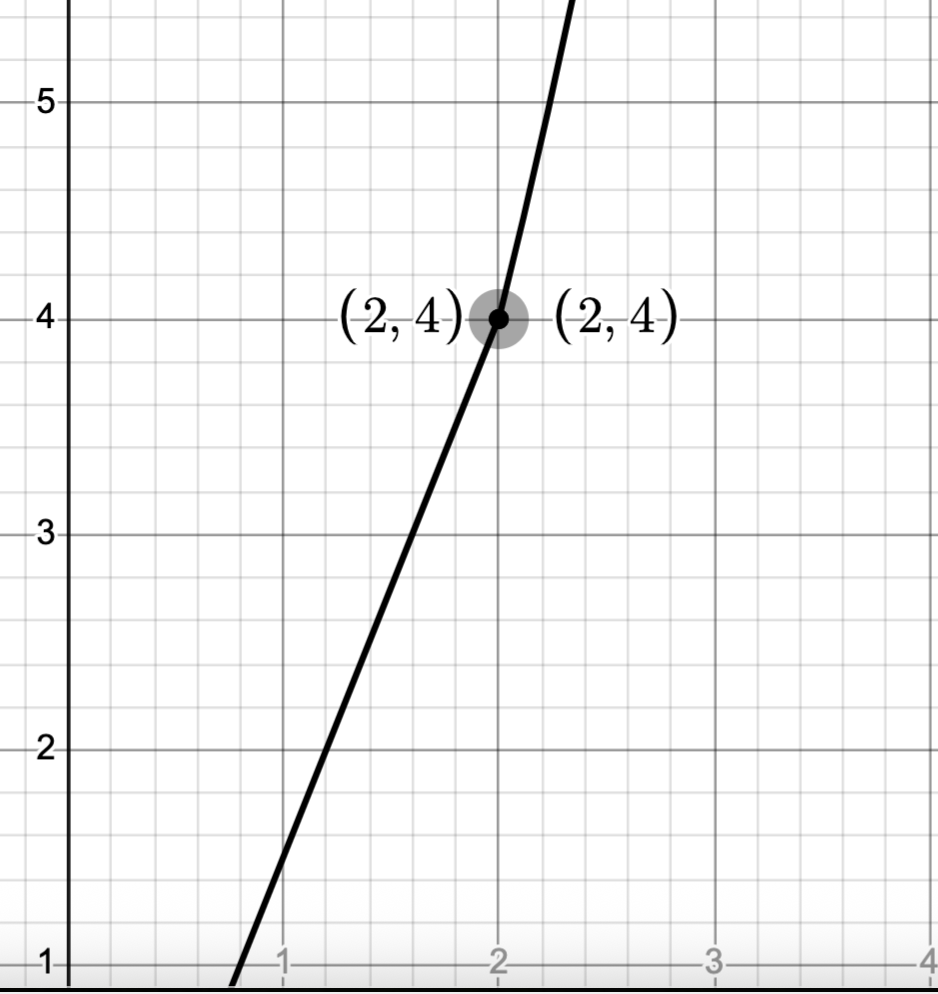
\includegraphics[width=3in]{./IntroLimitsGraphics/glued.png} \\
 
 $y = f(x)$ near $x = 2$ & $y = g(x)$ near $x = 2$  \\
 
 \end{tabular}
 
 \hfill \qed
 
 \end{center}

\end{enumerate}
\end{ex}

It is worth noting that despite each `piece' of the piecewise-defined function $f$ in Example \ref{piecewisecontex} being continuous, the pieces don't match up at $x=2$ causing what is called a\index{discontinuity ! jump} \textbf{discontinuity}.   A discontinuity is a place where a function is \textbf{not} continuous.  The particular variety of discontinuity appearing here  is usually called a `jump' discontinuity - a type of discontinuity belonging to a larger class of  `non-removable' or `essential' discontinuities.  We'll point out other types of discontinuities as we encounter them.\footnote{Probably in the footnotes because, after all, this is (supposedly) a \underline{pre}calculus book, not a Calculus book \ldots} 

\medskip

We close this section with an example that ties (most of) the fundamental concepts of limits and their calculations together.

\medskip

\begin{ex} \label{rationallimit}  Let  $f(x) =  \frac{x^2-2x-3}{x^2-1}$.  Find $\ds{\lim_{x \rightarrow -1} f(x)}$ analytically\footnote{i.e, using properties of limits} and interpret graphically.

\medskip

{\bf Solution.}  Since $f$ is a rational function, and rational functions are continuous on their domains, it's worth checking to see what happens when we attempt to find $f(-1)$.  We get  $f(-1) = \frac{(-1)^2 - 2(-1)-3}{(-1)^2-1} = \frac{0}{0},$ which is undefined because of the `$0$' in the denominator.  However, the `$0$' in the numerator signals to us\footnote{courtesy of the Factor Theorem (Theorem \ref{factorthm}) \ldots} there are common factors of $(x-(-1)) = (x+1)$ which will cancel and potentially help us determine the indeterminate form.  To that end, we simplify: $f(x) =  \frac{x^2-2x-3}{x^2-1} = \frac{(x-3)(x+1)}{(x-1)(x+1)} = \frac{(x-3)\cancel{(x+1)}}{(x-1)\cancel{(x+1)}} = \frac{x-3}{x-1}, \quad x \neq -1$. 

\medskip

That is, for all real numbers \textbf{except} $x = -1$, $\frac{x^2-2x-3}{x^2-1} = \frac{x-3}{x-1}$.   Since $\ds{\lim_{x \rightarrow -1} f(x)}$ is concerned only with what's happening \textbf{near} $x = -1$, but not with what's happening \textbf{at} $x = -1$, it seems reasonable to suggest that $\ds{\lim_{x \rightarrow -1} f(x) =  \lim_{x \rightarrow -1}}$  $\frac{x^2-2x-3}{x^2-1} =$  $\ds{\lim_{x \rightarrow -1}}$ $\frac{x-3}{x-1}$.

\medskip

Note that $x = -1$ is in the domain of the function $g(x) = \frac{x-3}{x-1}$, hence $g$  \textbf{is} continuous at $x = -1$.   This means $\ds{\lim_{x \rightarrow -1} g(x) = g(-1)}$, that is, $\ds{\lim_{x \rightarrow -1}}$ $\frac{x-3}{x-1} = \frac{-1-3}{-1-1} = 2$.

\medskip

Putting all of this work together, we get $\ds{\lim_{x \rightarrow -1} f(x) =   \lim_{x \rightarrow -1}}$ $ \frac{x-3}{x-1}  =  \frac{-1-3}{-1-1} = 2$.   Graphically, this means there is a hole in the graph of $f$ at the location $(-1,2)$.\footnote{Since $f(-1)$ is undefined but  $\ds{\lim_{x \rightarrow -1} f(x)}$ exists means the discontinuity here is classified as `removable.'  We can `remove' the discontinuity by `patching' the `hole' by defining $f(-1) = 2$. We do such repairs in Calculus.}  The table and graph below confirm our answer.\footnote{Note that depending on which graphing utility is used, the `hole' at $(-1,2)$ may or may not be immediately visible on the graph.}

\begin{center}

 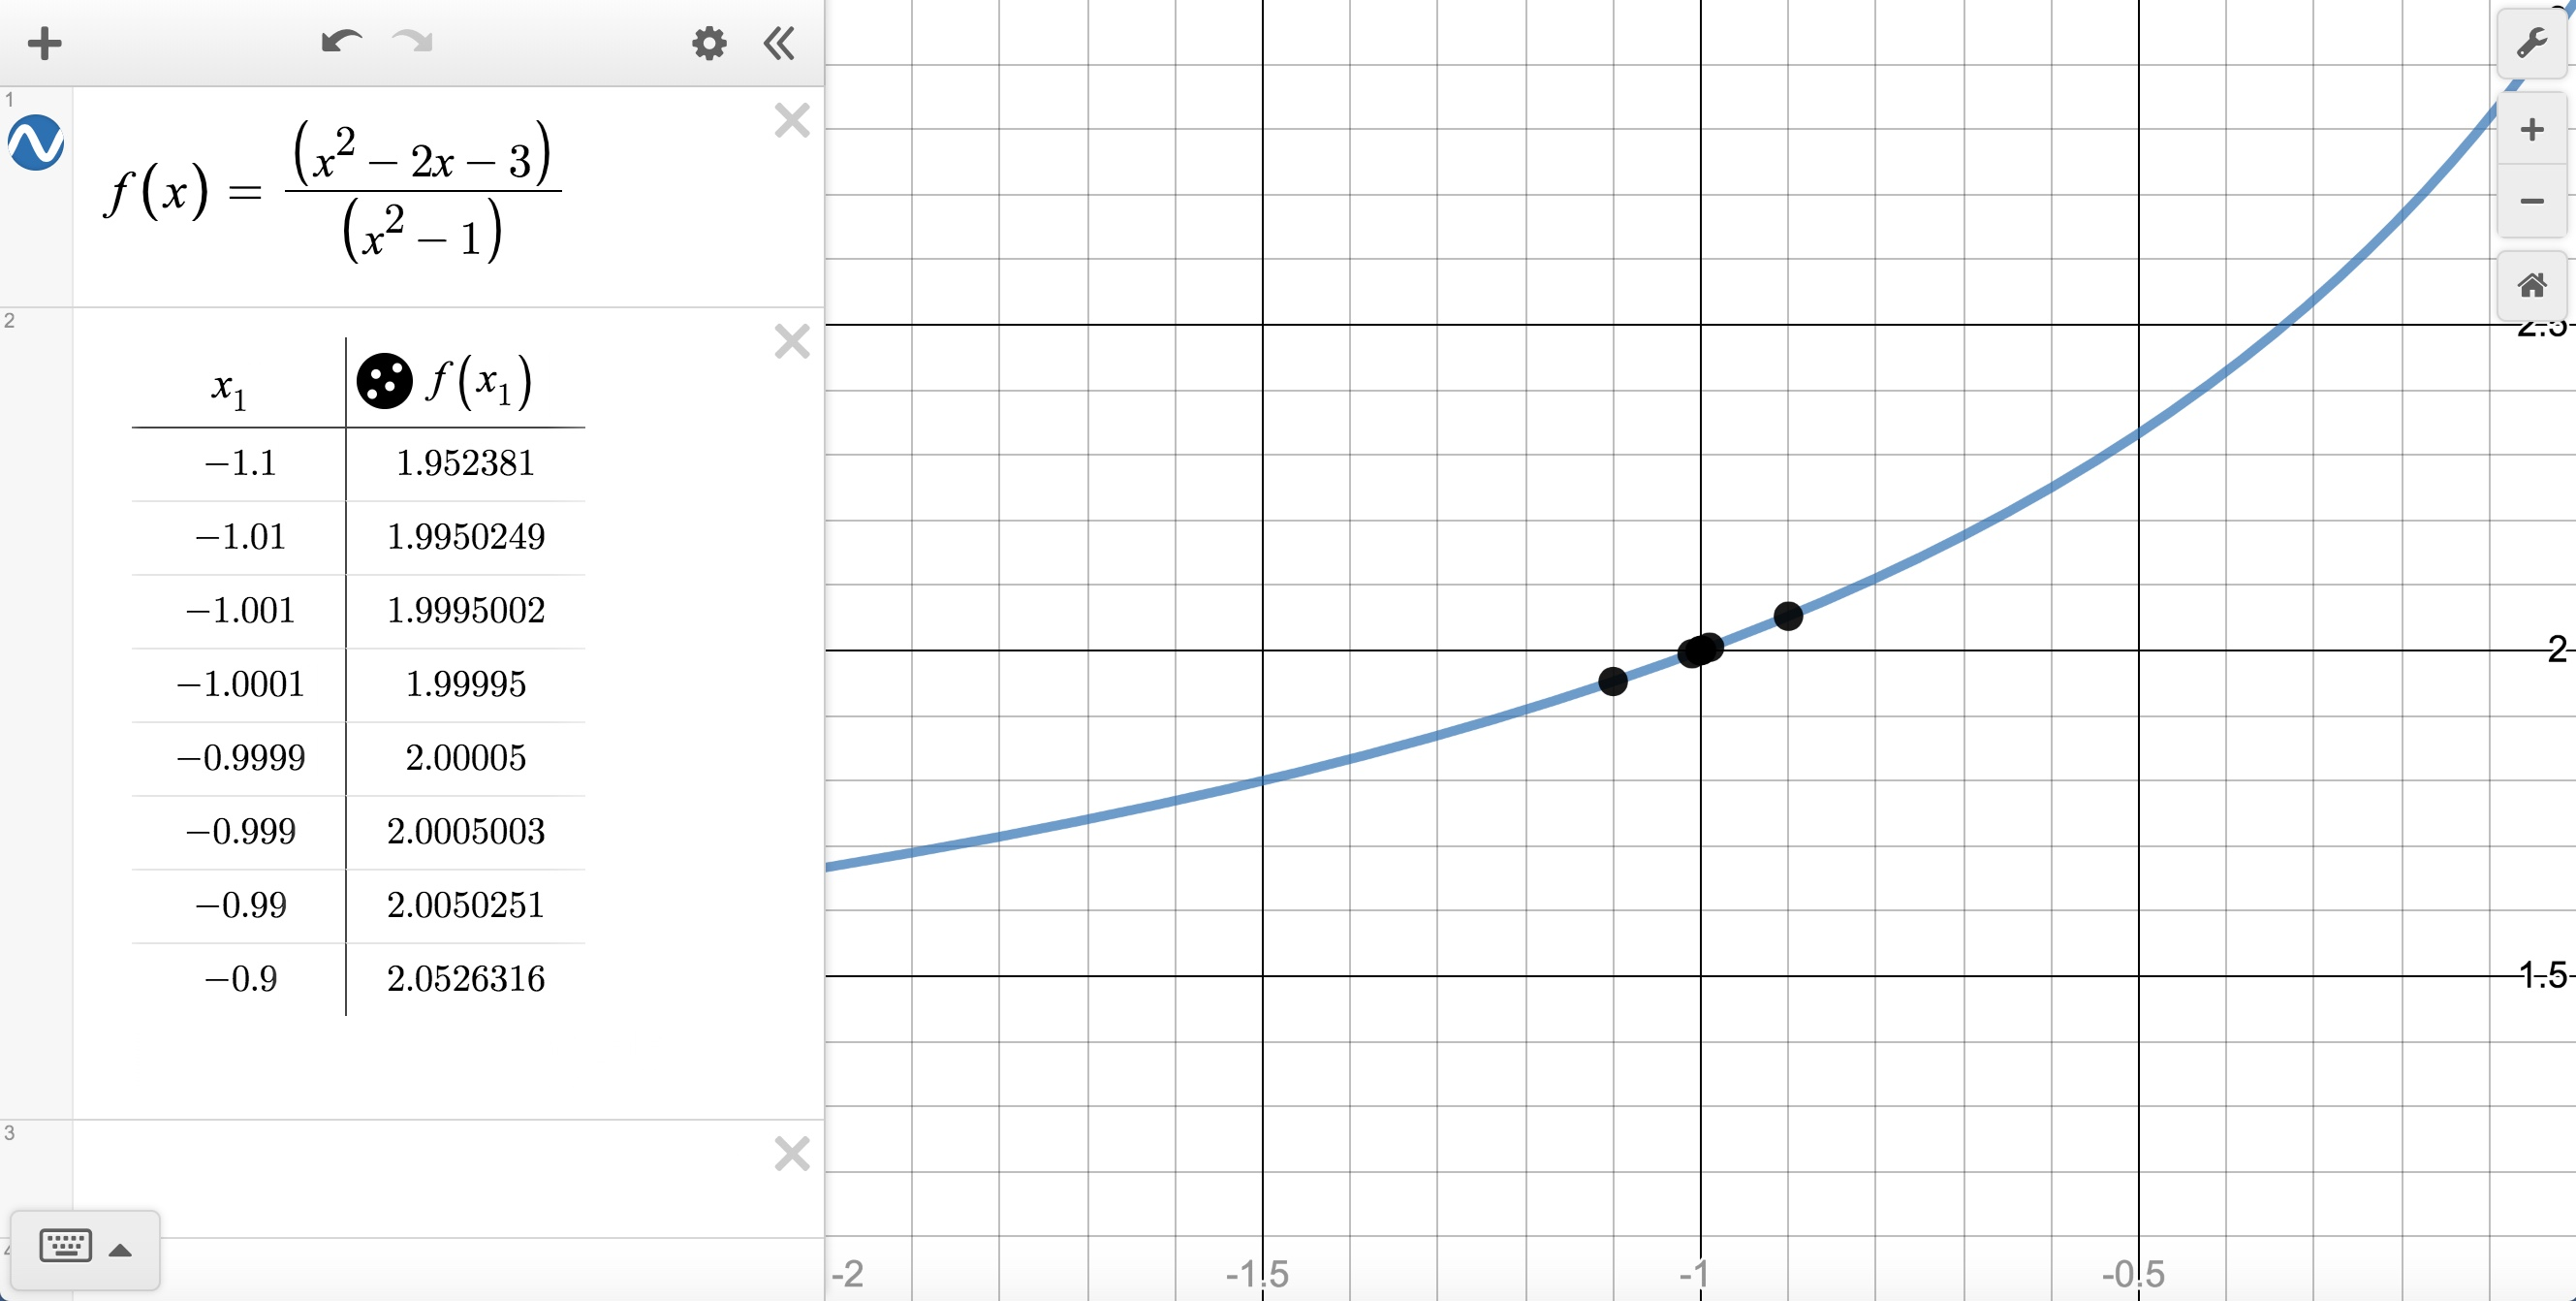
\includegraphics[width=5in]{./IntroLimitsGraphics/NearNegativeOne.jpeg} 
 
 $y = f(x)$ near $x = -1$

\end{center}

\hfill \qed



\end{ex}

\medskip

The above reasoning is sound and is true in general.  We'll be getting a lot of use out of the following:

\medskip

\colorbox{ResultColor}{\bbm

\begin{thm}  \label{limitsagree} If $f$ and $g$ are two functions which agree on an open interval containing $x = a$, except possibly at $x = a$, then if $\ds{\lim_{x \rightarrow a} g(x)}$ exists, $\ds{ \lim_{x \rightarrow a} f(x) = \lim_{x \rightarrow a} g(x)}$.


\end{thm}
\ebm}







\newpage

\subsection{Exercises}
%% SKIPPED %% \label{ExercisesforIntroLimits}

\begin{enumerate}

\item  Consider the complete graph of the function $f$ below.  Use the graph to find the indicated values.

\smallskip

If a limit fails to exist, state that is the case  or use the symbols `$\infty$' or `$-\infty$' appropriately.
 
 \smallskip
 
 \textbf{NOTE:}  The graph has a vertical asymptote $x=3$.  

\begin{center}

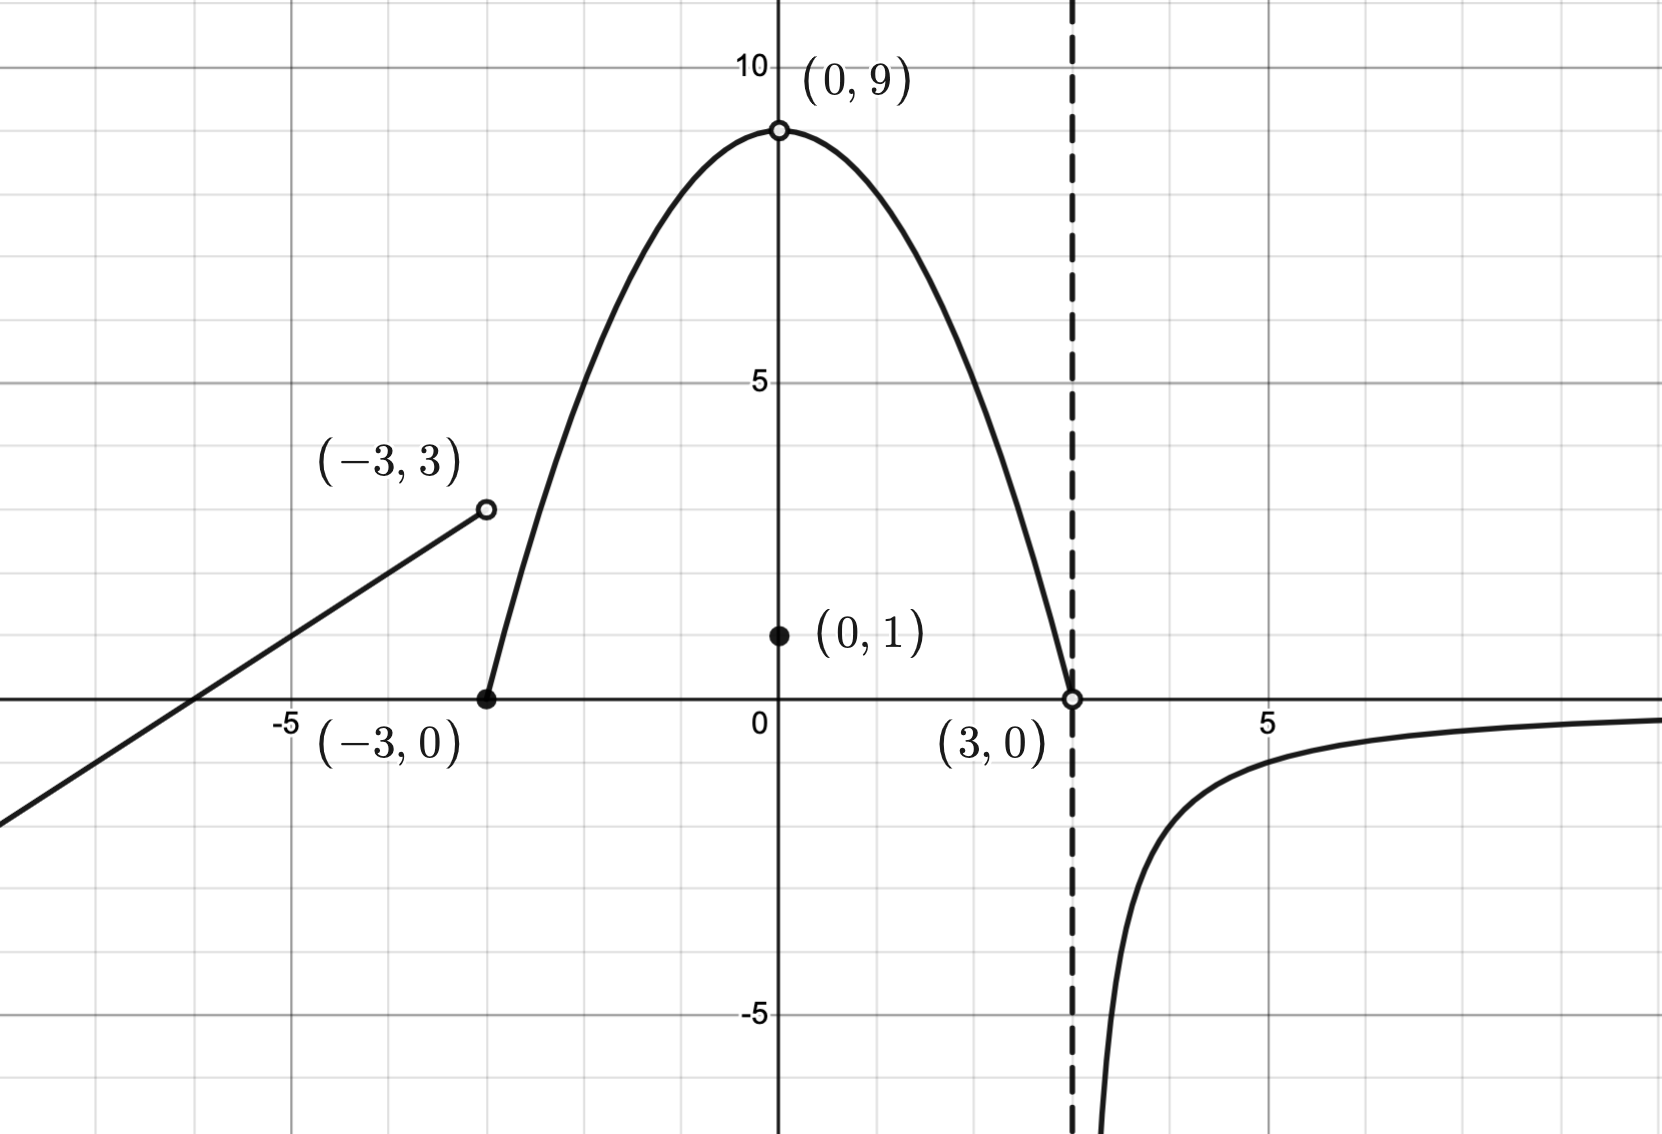
\includegraphics[width=5.5in]{./IntroLimitsGraphics/M2500TH01.png}

\end{center}

\bigskip

\begin{multicols}{4}

\begin{itemize}

\item $\ds{\lim_{x \rightarrow -3^{-}} f(x)}$

\item $\ds{\lim_{x \rightarrow -3^{+}} f(x)}$

\item $\ds{\lim_{x \rightarrow -3} f(x)}$

\item $f(-3)$

\end{itemize}

\end{multicols}

\bigskip

\begin{multicols}{4}

\begin{itemize}

\item $\ds{\lim_{x \rightarrow 0} f(x)}$

\item  $f(0)$

\item $\ds{\lim_{x \rightarrow 3^{-}} f(x)}$

\item $\ds{\lim_{x \rightarrow 3^{+}} f(x)}$
\end{itemize}

\end{multicols}

\bigskip


\item\label{twosidedonesidedlimitexistexercise}  \begin{enumerate}  \item  Explain why if $\ds{\lim_{x \rightarrow a} f(x)}$ exist, then so do $\ds{\lim_{x \rightarrow a^{-}} f(x)}$ and $\ds{\lim_{x \rightarrow a^{+}} f(x)}$.

\item   Find an instance\footnote{There are a few examples to be found in Example \ref{limitfromgraphex} \ldots}  where   $\ds{\lim_{x \rightarrow a^{-}} f(x)}$ and $\ds{\lim_{x \rightarrow a^{+}} f(x)}$ both exist but $\ds{\lim_{x \rightarrow a} f(x)}$ does not.

\end{enumerate}

\item  Consider the complete graph of the function $g$ below.  Use the graph to find the indicated values.

\smallskip


If a limit fails to exist, state that is the case  or use the symbols `$\infty$' or `$-\infty$' appropriately.
  
\smallskip

 
 \textbf{NOTE:}  The graph has a vertical asymptote $x=-2$ and a horizontal asymptote $y = 1$.  



\begin{center}

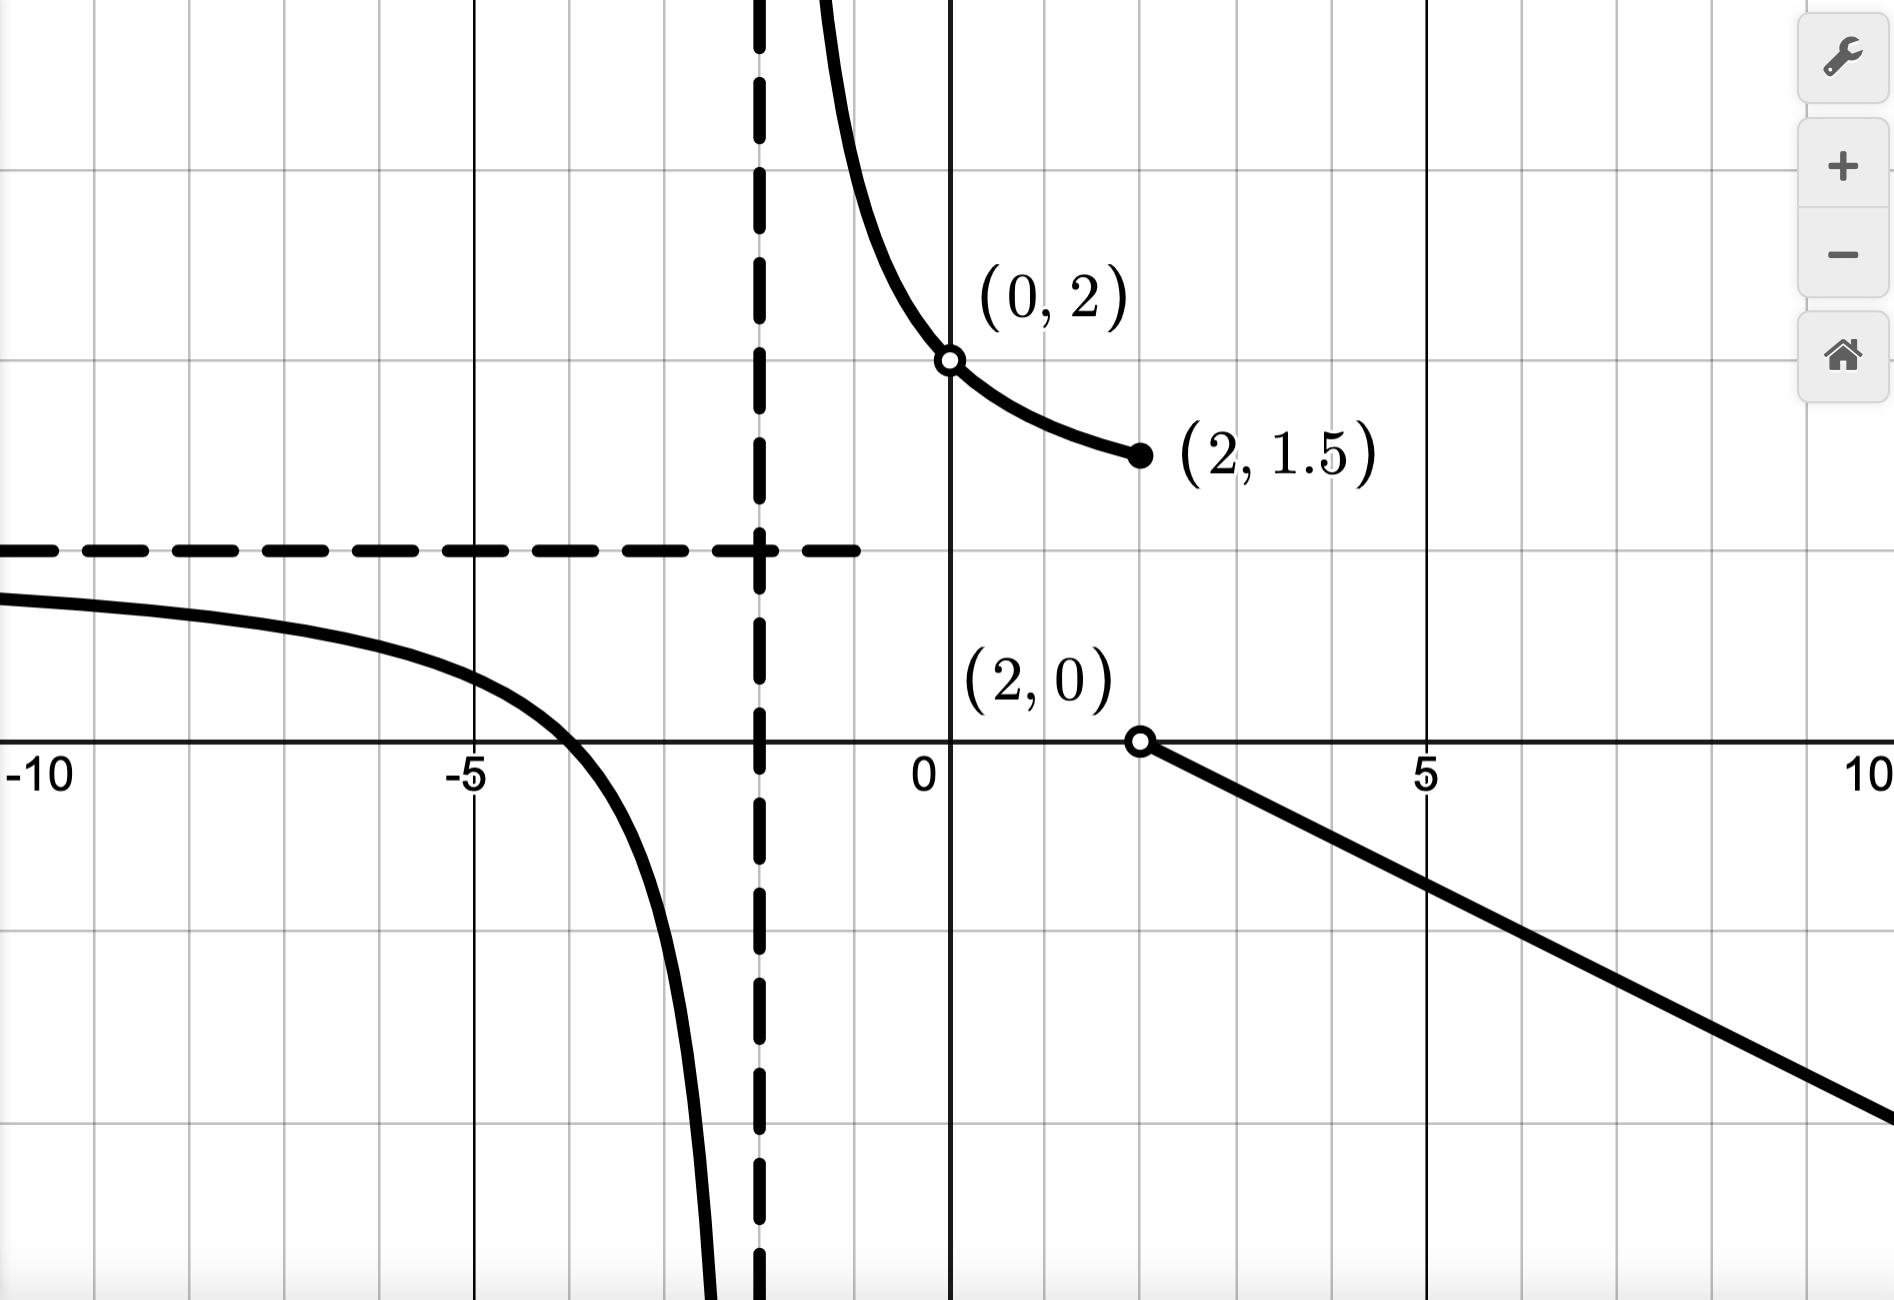
\includegraphics[width=5.5in]{./IntroLimitsGraphics/M2500_T01_Sp25_a.png}

\end{center}

\bigskip

\begin{multicols}{4}

\begin{itemize}

\item $\ds{\lim_{x \rightarrow -\infty} g(x)}$

\item $\ds{\lim_{x \rightarrow -2^{-}} g(x)}$

\item $\ds{\lim_{x \rightarrow -2^{+}} g(x)}$

\item  $\ds{\lim_{x \rightarrow \infty} g(x)}$

\end{itemize}

\end{multicols}

\bigskip

\begin{multicols}{4}

\begin{itemize}

\item $\ds{\lim_{x \rightarrow 0} g(x)}$

\item $\ds{\lim_{x \rightarrow 2^{-}} g(x)}$

\item  $g(2)$

\item $\ds{\lim_{x \rightarrow 2^{+}} g(x)}$
\end{itemize}

\end{multicols}

\bigskip

\setcounter{HW}{\value{enumi}}
\end{enumerate}

For Exercises \ref{factorcancelfirst} - \ref{factorcancellast}, find the limit analytically using Exercise \ref{rationallimit} as a guide.  If a limit fails to exist, state that is the case  or use the symbols `$\infty$' or `$-\infty$' appropriately.
 
\begin{multicols}{3}

\begin{enumerate}
\setcounter{enumi}{\value{HW}}

\item\label{factorcancelfirst}  $\ds{\lim_{x \rightarrow 2} \dfrac{2x^2+x-3}{x^2-1}}$
  
\item  $\ds{\lim_{x \rightarrow 1} \dfrac{2x^2+x-3}{x^2-1}}$

\item   $\ds{\lim_{x \rightarrow -1} \dfrac{2x^2+x-3}{x^2-1}}$

\setcounter{HW}{\value{enumi}}
\end{enumerate}

\end{multicols}

\begin{multicols}{3}

\begin{enumerate}
\setcounter{enumi}{\value{HW}}

\item   $\ds{\lim_{x \rightarrow -1^{+}} \dfrac{2x^2+x-3}{x^2-1}}$

\item  $\ds{\lim_{x \rightarrow 3} \dfrac{x^2-3x}{x^2-x-6}}$

\item\label{factorcancellast}  $\ds{\lim_{x \rightarrow 3} \dfrac{x^2-6x}{x^2-6x+9}}$

\setcounter{HW}{\value{enumi}}
\end{enumerate}

\end{multicols}

For Exercises \ref{abscancelfirst} - \ref{abscancellast}, use the piecewise definition of absolute value, Definition \ref{absolutevaluepiecewise} to help you find the limit analytically.    If a limit fails to exist, state that is the case  or use the symbols `$\infty$' or `$-\infty$' appropriately.

\begin{multicols}{2}
\begin{enumerate}
\setcounter{enumi}{\value{HW}}

\item\label{abscancelfirst} $\ds{ \lim_{x \rightarrow 3^{-}} \dfrac{|3x - x^2| }{x-3}}$     

\item\label{abscancellast}  $\ds{\lim_{x \rightarrow 2^{+}} \dfrac{|6-3x|}{x^2-4x+4}}$

\setcounter{HW}{\value{enumi}}
\end{enumerate}
\end{multicols}

For Exercises \ref{complexcancelfirst} - \ref{complexcancellast}, simplify the complex fraction in order to help you find the limit analytically.\footnote{A review of Section \ref{AppRatExpEqus} may be in order.}  If a limit fails to exist, state that is the case  or use the symbols `$\infty$' or `$-\infty$' appropriately.

\begin{multicols}{3}
\begin{enumerate}
\setcounter{enumi}{\value{HW}}

\item\label{complexcancelfirst}  $\ds{\lim_{x \rightarrow 1} \dfrac{\dfrac{x}{x-2} +1}{x-1}}$

\item $\ds{ \lim_{x \rightarrow 2} \dfrac{\dfrac{2x}{x+2}  -1}{x-2} }$ 
     
\item\label{complexcancellast} $\ds{ \lim_{h \rightarrow 0} \dfrac{\dfrac{1}{2(x+h) - 1}  - \dfrac{1}{2x-1} }{h} }$ 

\setcounter{HW}{\value{enumi}}
\end{enumerate}
\end{multicols}

For Exercises \ref{radicalcancelfirst} - \ref{radicalcancellast}, rationalize the numerator of the fraction in order to help you find the limit analytically.\footnote{A review of Section \ref{rationalizingdenomandnumer} may be in order.} If a limit fails to exist, state that is the case  or use the symbols `$\infty$' or `$-\infty$' appropriately.


\begin{multicols}{3}
\begin{enumerate}
\setcounter{enumi}{\value{HW}}

 \item\label{radicalcancelfirst}  $\ds{ \lim_{x \rightarrow -1} \dfrac{\sqrt{x+5} - 2 }{x+1} }$  
   
 \item   $\ds{\lim_{h \rightarrow 0} \dfrac{\sqrt{4+h} - 2}{h}}$

\item\label{radicalcancellast} $\ds{ \lim_{h \rightarrow 0} \dfrac{\sqrt{2x+2h-1} - \sqrt{2x-1} }{h} }$  

\setcounter{HW}{\value{enumi}}
\end{enumerate}
\end{multicols}


 In Exercises \ref{limitatinfinityfirst} - \ref{limitatinfinitylast},  find the limit analytically.  Use the symbols `$\infty$' and `$-\infty$' as appropriate.

 \begin{multicols}{3}
\begin{enumerate}
\setcounter{enumi}{\value{HW}}

\item\label{limitatinfinityfirst}   $\ds{ \lim_{x \rightarrow \infty} \dfrac{3x-4}{2x+1}}$

\item $\ds{ \lim_{x \rightarrow -\infty}  \dfrac{1-2x}{x-5}}$ 

\item $\ds{ \lim_{x \rightarrow -\infty}\dfrac{2x-1}{x^2+4}}$

\setcounter{HW}{\value{enumi}}
\end{enumerate}
\end{multicols}

 \begin{multicols}{3}
\begin{enumerate}
\setcounter{enumi}{\value{HW}}
\item $\ds{ \lim_{x \rightarrow \infty}\dfrac{\sqrt{4x^2+x-1}}{1-x}}$

\item $\ds{ \lim_{x \rightarrow -\infty}\dfrac{\sqrt{4x^2+x-1}}{1-x}}$

\item\label{limitatinfinitylast}  $\ds{ \lim_{x \rightarrow \infty} \dfrac{x^2+2x+3}{4-x}}$.

\setcounter{HW}{\value{enumi}}
\end{enumerate}
\end{multicols}

\begin{enumerate}
\setcounter{enumi}{\value{HW}}

\item  Let $f(x) = \dfrac{x}{\lfloor x \rfloor}$  where `$\lfloor x \rfloor$'  is the greatest integer (or floor) function.\footnote{See Example \ref{greatestintegerdefn} in Section \ref{ConstantandLinearFunctions} for review, if needed.} 

\smallskip

Fill in the blanks below to help you analyze $\ds{ \lim_{x \rightarrow 0} f(x)}$.

\smallskip

\begin{enumerate}

\item  If $-1 < x < 0$, then $\lfloor x \rfloor = \underline{\hspace{1in}}$. So we can rewrite $f(x) = \dfrac{x}{\lfloor x \rfloor} =  \underline{\hspace{1in}}$.

\item  Using part (a), we can find  $\ds{ \lim_{x \rightarrow 0^{-}} f(x) =  \lim_{x \rightarrow 0^{-}}  \underline{\hspace{1in}} =  \underline{\hspace{1in}} }$.

\item  If $0 < x < 1$, then $\lfloor x \rfloor = \underline{\hspace{1in}}$, hence $f(x) = \dfrac{x}{\lfloor x \rfloor}$ does not exist as $x \rightarrow 0^{+}$.

\item  Putting parts (b) and (c) together, we have that   $\ds{ \lim_{x \rightarrow 0} f(x)  \qquad \underline{\hspace{1.5in}}}$

\item  Graph $f(x) = \dfrac{x}{\lfloor x \rfloor}$ on desmos near $x = 0$ to confirm your answers.

\end{enumerate}

\newpage

\item  Sketch the graph of a function which satisfies all of the following criteria:

\bigskip

\begin{multicols}{4}

\begin{itemize}

\item $\ds{\lim_{x \rightarrow -\infty}  f(x) = \infty}$

\item $\ds{\lim_{x \rightarrow 4^{-}} f(x) = 6}$

\item $\ds{\lim_{x \rightarrow 4^{+}} f(x) = - \infty}$

\item $\ds{\lim_{x \rightarrow \infty}  f(x) =0}$

\end{itemize}

\end{multicols}

\item Sketch the graph of a function $f$  which satisfies all of the following criteria:

\bigskip

\begin{multicols}{3}

\begin{itemize}

\item $\ds{\lim_{x \rightarrow -\infty} f(x) = 2}$

\item $\ds{\lim_{x \rightarrow 0^{-}} f(x) = \infty}$

\item $\ds{\lim_{x \rightarrow 0^{+}} f(x) = -\infty}$

\end{itemize}

\end{multicols}

\bigskip

\begin{multicols}{3}

\begin{itemize}

\item $\ds{\lim_{x \rightarrow 2^{-}} f(x) = 3}$

\item $\ds{\lim_{x \rightarrow 2^{+}} f(x) =0}$

\item $\ds{\lim_{x \rightarrow \infty} f(x) = -\infty}$

\end{itemize}

\end{multicols}


\item\label{onesidedcontinuityexercise}  A function is said to be \index{continuous from the left}\index{continuous ! from the left}\index{one-sided continuity}\index{continuity ! one sided}\textbf{continuous from the left} at $x=a$ if $\ds{\lim_{x \rightarrow a^{-}} f(x) = f(a)}$.  Likewise, a function is said to be \index{continuous from the right}\index{continuous ! from the right}\index{one-sided continuity}\index{continuity ! one sided}\textbf{continuous from the right} at $x=a$ if $\ds{\lim_{x \rightarrow a^{+}} f(x) = f(a)}$.

\begin{enumerate}

\item   Explain why $r(x) = \sqrt{5-x}$ is not continuous at $x = 5$.  Is $r$ continuous from the left at $x=5$?  From the right?  Explain.

\item  Explain why the floor function\footnote{See Example \ref{greatestintegerdefn} in Section \ref{ConstantandLinearFunctions} for review, if needed.} $F(x) = \lfloor x \rfloor$ is not continuous at $x = 117$.   Is $F$ continuous from the left at $x=117$?  From the right?  Explain.

\item  If a function $f$ is continuous at $x = a$, explain why $f$ is continuous from both the left and the right at $x = a$.  Is the converse true?  That is, if $f$ is continuous from both the left and the right at $x = a$, is $f$ continuous at $x=a$?  

\item  Compare and contrast your answers in this exercise to those in Exercise \ref{twosidedonesidedlimitexistexercise}.


\end{enumerate}


\item  Consider the table of values below:

\[ \begin{array}{|r|c|} 

\hline

x & f(x)  \\    \hline 

-0.001  &  1.9 \\   [1ex]  \hline 

-0.0001 & 1.99 \\ [1ex]  \hline

-0.00001 & 1.999\\  [1ex] \hline

-0.000001 & 1.9999 \\ [1ex]  \hline

0.000001 & -10000\\  [1ex]   \hline

0.00001 & -1000 \\ [1ex]  \hline

0.0001 & - 100 \\  [1ex] \hline

0.001 & -10 \\ [1ex]  \hline


\end{array} \]

It turns out that $\ds{\lim_{x \rightarrow 0} f(x) = 117}$.  How is this possible assuming the data in the table is correct?

\item  In this exercise, we use Definition \ref{infinitelimitsatinfinity} to prove $\ds{\lim_{x \rightarrow \infty} x^3 = \infty}$ and $\ds{\lim_{x \rightarrow -\infty} x^3 = -\infty}$:


\begin{enumerate}

\item  Solve the following inequalities:

\begin{multicols}{4}

\begin{itemize}

\item  $x^3 > 1000$

\item  $x^3 > 100000$

\item  $x^3 > 10^{99}$

\item  $x^3 > N$

\end{itemize}

\end{multicols}

\item  Show that for $N > 0$, if $x > \sqrt[3]{N}$, then $x^3 > N$.  Write a sentence (or two!) which uses your work and Definition \ref{infinitelimitsatinfinity} to prove $\ds{\lim_{x \rightarrow \infty} x^3 = \infty}$.

\item  Repeat a similar argument to prove $\ds{\lim_{x \rightarrow -\infty} x^3 = -\infty}$

\end{enumerate}
 
\end{enumerate}

\newpage

\subsection{Answers}

\begin{enumerate}

\item  \begin{multicols}{4} \begin{itemize} \item $\ds{\lim_{x \rightarrow -3^{-}} f(x) = 3}$

\item $\ds{\lim_{x \rightarrow -3^{+}} f(x) = 0}$

\item $\ds{\lim_{x \rightarrow -3} f(x)}$ d.n.e.

\item $f(-3) = 0$

\end{itemize}

\end{multicols}

\bigskip

\begin{multicols}{4}

\begin{itemize}

\item $\ds{\lim_{x \rightarrow 0} f(x) = 9}$

\item  $f(0)$

\item $\ds{\lim_{x \rightarrow 3^{-}} f(x) = 0}$

\item $\ds{\lim_{x \rightarrow 3^{+}} f(x) = -\infty}$
\end{itemize}

\end{multicols}

\bigskip


\item  \begin{enumerate}  \item  If $\ds{\lim_{x \rightarrow a} f(x)}$ exists, say $\ds{\lim_{x \rightarrow a} f(x) = L}$ then the $f(x)$ values approach  $L$  as $x \rightarrow a$ from both directions.  Hence both one-sided limits exist.  In particular,  $\ds{\lim_{x \rightarrow a^{-}} f(x) = L}$ and $\ds{\lim_{x \rightarrow a^{+}} f(x) = L}$.

\item  In Example \ref{limitfromgraphex},  $\ds{\lim_{x \rightarrow -1^{-}} f(x)  = 0}$ and $\ds{\lim_{x \rightarrow -1^{+}} f(x) = 4}$ both exist but $\ds{\lim_{x \rightarrow -1} f(x)}$ does not because the two one-sided limits are not equal.

\end{enumerate}

\item  \begin{multicols}{4} \begin{itemize} \item $\ds{\lim_{x \rightarrow -\infty} g(x) = 1}$

\item $\ds{\lim_{x \rightarrow -2^{-}} g(x) = -\infty}$

\item $\ds{\lim_{x \rightarrow -2^{+}} g(x) = \infty}$

\item  $\ds{\lim_{x \rightarrow \infty} g(x) = -\infty}$

\end{itemize}

\end{multicols}

\bigskip

\begin{multicols}{4}

\begin{itemize}

\item $\ds{\lim_{x \rightarrow 0} g(x) = 2}$

\item $\ds{\lim_{x \rightarrow 2^{-}} g(x) = 1.5}$

\item  $g(2) = 1.5$

\item $\ds{\lim_{x \rightarrow 2^{+}} g(x) = 0}$
\end{itemize}

\end{multicols}

\bigskip

\setcounter{HW}{\value{enumi}}
\end{enumerate}
 


\begin{enumerate}
\setcounter{enumi}{\value{HW}}

\item  $\ds{\lim_{x \rightarrow 2} \dfrac{2x^2+x-3}{x^2-1} = \frac{7}{3}}$

\medskip
  
\item  $\ds{\lim_{x \rightarrow 1} \dfrac{2x^2+x-3}{x^2-1} = \frac{5}{2}}$

\medskip

\item   $\ds{\lim_{x \rightarrow -1} \dfrac{2x^2+x-3}{x^2-1}}$ does not exist

\medskip

\setcounter{HW}{\value{enumi}}
\end{enumerate}



\begin{enumerate}
\setcounter{enumi}{\value{HW}}

\item   $\ds{\lim_{x \rightarrow -1^{+}} \dfrac{2x^2+x-3}{x^2-1} = \infty}$

\medskip

\item  $\ds{\lim_{x \rightarrow 3} \dfrac{x^2-3x}{x^2-x-6} = \frac{3}{5}}$


\medskip

\item  $\ds{\lim_{x \rightarrow 3} \dfrac{x^2-6x}{x^2-6x+9} = -\infty}$

\medskip

\setcounter{HW}{\value{enumi}}
\end{enumerate}




\begin{enumerate}
\setcounter{enumi}{\value{HW}}

\item  $\ds{ \lim_{x \rightarrow 3^{-}} \dfrac{|3x - x^2| }{x-3} = -3}$ 

\medskip    

\item $\ds{\lim_{x \rightarrow 2} \dfrac{|6-3x|}{x^2-4x+4} = \infty}$

\medskip

\setcounter{HW}{\value{enumi}}
\end{enumerate}

\begin{enumerate}
\setcounter{enumi}{\value{HW}}

\item  $\ds{\lim_{x \rightarrow 1} \dfrac{\dfrac{x}{x-2} +1}{x-1} = -2}$

\medskip

\item $\ds{ \lim_{x \rightarrow 2} \dfrac{\dfrac{2x}{x+2}  -1}{x-2}  = \frac{1}{4}}$ 

\medskip
     
\item $\ds{ \lim_{h \rightarrow 0} \dfrac{\dfrac{1}{2(x+h) - 1}  - \dfrac{1}{2x-1} }{h} = -\frac{2}{(2x-1)^2} }$ 

\medskip

\setcounter{HW}{\value{enumi}}
\end{enumerate}

\begin{enumerate}
\setcounter{enumi}{\value{HW}}

 \item  $\ds{ \lim_{x \rightarrow -1} \dfrac{\sqrt{x+5} - 2 }{x+1}  = \frac{1}{4}}$  
 
 \medskip
 
 \item $\ds{\lim_{h \rightarrow 0} \dfrac{\sqrt{4+h} - 2}{h}} = \frac{1}{4}$
 
 \medskip
   
 \item  $\ds{ \lim_{h \rightarrow 0} \dfrac{\sqrt{2x+2h-1} - \sqrt{2x-1} }{h}  = \frac{1}{\sqrt{2x-1}}}$  

\medskip

\setcounter{HW}{\value{enumi}}
\end{enumerate}

\begin{enumerate}
\setcounter{enumi}{\value{HW}}

\item  $\ds{ \lim_{x \rightarrow \infty} \dfrac{3x-4}{2x+1} = \frac{3}{2}}$

\medskip

\item $\ds{ \lim_{x \rightarrow -\infty}  \dfrac{1-2x}{x-5} = -2}$ 

\medskip

\item $\ds{ \lim_{x \rightarrow -\infty}\dfrac{2x-1}{x^2+4} = 0}$

\medskip

\setcounter{HW}{\value{enumi}}
\end{enumerate}

\begin{enumerate}
\setcounter{enumi}{\value{HW}}
\item $\ds{ \lim_{x \rightarrow \infty}\dfrac{\sqrt{4x^2+x-1}}{1-x} = -2}$

\medskip

\item $\ds{ \lim_{x \rightarrow -\infty}\dfrac{\sqrt{4x^2+x-1}}{1-x}  = 2}$

\medskip

\item $\ds{ \lim_{x \rightarrow \infty} \dfrac{x^2+2x+3}{4-x} = -\infty}$

\medskip

\setcounter{HW}{\value{enumi}}
\end{enumerate}


\begin{enumerate}
\setcounter{enumi}{\value{HW}}

\item   \begin{enumerate}

\item  If $-1 < x < 0$, then $\lfloor x \rfloor = -1$. So we can rewrite $f(x) = \dfrac{x}{\lfloor x \rfloor} = -x$.

\smallskip

\item  Using part (a), we can find  $\ds{ \lim_{x \rightarrow 0^{-}} f(x) =  \lim_{x \rightarrow 0^{-}} -x = 0}$.

\smallskip

\item  If $0 < x < 1$, then $\lfloor x \rfloor =0$, hence $f(x) = \dfrac{x}{\lfloor x \rfloor}$ does not exist as $x \rightarrow 0^{+}$.

\smallskip

\item  Putting parts (b) and (c) together, we have that   $\ds{ \lim_{x \rightarrow 0} f(x)}$   does not exist.

\smallskip

\end{enumerate}

\item Answers vary.

\item  Answers vary.

\item \begin{enumerate} \item    The function $r(x) = \sqrt{5-x}$ is not continuous at $x = 5$ since $r$ is undefined if $x>5$, so $\ds{\lim_{x \rightarrow 5^{+}} r(x)}$ does not exist. However, $r$ is continuous from the left at $x = 5$ since 

$\ds{\lim_{x \rightarrow 5^{-}} r(x) =  \lim_{x \rightarrow 5^{-}} \sqrt{5-x} = 0 = \sqrt{5-5} = r(5)}$.

\smallskip

\item  The function  $F(x) = \lfloor x \rfloor$ is not continuous at $x = 117$ since $\ds{\lim_{x \rightarrow 117^{-}} \lfloor x \rfloor = 116}$ but $\ds{\lim_{x \rightarrow 117^{+}} \lfloor x \rfloor = 117}$.  However, $F$ is continuous from the right at $x = 117$ since $\ds{\lim_{x \rightarrow 117^{+}} \lfloor x \rfloor = 117 = \lfloor 117 \rfloor = F(117)}$. 

\smallskip

\item If $f$ is continuous at $x=a$, then $\ds{\lim_{x \rightarrow a} f(x) = f(a)}$.  This means  $\ds{\lim_{x \rightarrow a^{-}} f(x) = f(a)}$ and  $\ds{\lim_{x \rightarrow a^{+}} f(x) = f(a)}$, so $f$ is continuous from both directions at $x=a$. The converse is also true since  ff $\ds{\lim_{x \rightarrow a^{-}} f(x) = f(a)}$ and  $\ds{\lim_{x \rightarrow a^{+}} f(x) = f(a)}$, then $\ds{\lim_{x \rightarrow a} f(x) = f(a)}$.

\smallskip

\item  The difference between the scenario here and that in Exercise \ref{twosidedonesidedlimitexistexercise} is that here, we know what each of the one-sided limits are: $f(a)$. They can't be different numbers like they could be in  Example \ref{limitfromgraphex}

\smallskip

\end{enumerate}


\item  We are told nothing of the function on the interval $(-0.000001, 0.000001 )$ so the function has plenty of opportunities to approach $117$.  


\item \begin{enumerate}

\item \begin{itemize} \item  $x^3 > 1000$ for $x > 10$.

\item  $x^3 > 1000000$ for $x > 100$.

\item  $x^3 > 10^{99}$ for $x > 10^{33}$.

\item  $x^3 > N$ for $x > \sqrt[3]{N}$.

\end{itemize}


\item If $x > \sqrt[3]{N}$, then $x^3 > \left(\sqrt[3]{N} \right)^3 = N$.  Per  Definition \ref{infinitelimitsatinfinity}, given $N>0$, choose $M = \sqrt[3]{N}$.  If $x > M$, then $x^3 > M^3 = N$. Hence,  $\ds{\lim_{x \rightarrow \infty} x^3 = \infty}$.

\smallskip

\item Given $N<0$, choose $M = \sqrt[3]{N}$.  If $x< M$, then $x^3 < M^3 = \left(\sqrt[3]{N}\right)^3 = N$.  Hence,   $\ds{\lim_{x \rightarrow -\infty} x^3 = -\infty}$.

\end{enumerate}
 
\end{enumerate}


\closegraphsfile

\end{document}
